\documentclass[10pt]{article}
\usepackage{indentfirst}
\usepackage{hyperref}
\usepackage[dvips]{graphicx}
\usepackage{pst-plot}
\usepackage{mathrsfs}
\usepackage{epic,eepic}
\usepackage{amsfonts}
\usepackage{amsmath,amssymb}
\usepackage{bm}
\usepackage{enumitem}
\usepackage{subcaption}
\usepackage{braket}
\usepackage{tabto}
% set up paper size
\setlength{\textwidth}{17.59cm}
\setlength{\marginparsep}{0pt}
\setlength{\marginparwidth}{0pt}
\setlength{\textheight}{24.05cm}
\setlength{\headheight}{0pt}
\setlength{\headsep}{0pt}
\setlength{\oddsidemargin}{-0.04cm}
\setlength{\topmargin}{-.04cm}
\usepackage{pdfpages} 

\renewcommand{\baselinestretch}{1.1}
\DeclareMathOperator{\sgn}{sgn}

\newcommand{\dagg}[1]{\ensuremath #1^\dag}

\newcommand{\tbd}[1]{{\color{red}#1}}

\begin{document}

\thispagestyle{empty}

     \begin{center}
     \rule{\linewidth}{1mm}     
           \Huge From Quarks to Stars: A Quantum Computing Approach to the Nuclear Many-Body Problem
     \rule{\linewidth}{1mm}
     \end{center}
     \vspace*{\stretch{2}}
 \begin{center}
 \begin{figure}[hb]
 \includegraphics[scale=0.9]{Figures/NP_Collaboration.png}
 \end{figure}
 \end{center}
\newpage
\title{DOE Quantum Horizons: \\ QIS Research and Innovation for Nuclear Science}
\maketitle
\rule{\linewidth}{1mm}
\begin{flushleft}
{\bf Title: From Quarks to Stars: A Quantum Computing Approach to the Nuclear Many-Body Problem}\newline
Institution: Facility for Rare Isotope Beams and Michigan State University\newline
Address: 640 S.~Shaw Lane, East Lansing, MI 48824\newline
Administrative point of Contact: Chris West, westc@frib.msu.edu (517-908-7757) \newline
Lead Principal Investigator: Morten Hjorth-Jensen\newline
DOE Funding Opportunity Announcement (FOA) Number: DE-FOA-0002110\newline
FOA type: Initial\newline
CDFA Number: 81.049\newline
DOE/Office of Science Program Office: {\bf Nuclear Physics}\newline
DOE/Office of Science Program Office Technical Contact: Dr. Gulshan Rai (301-903-4702), gulshan.rai@science.doe.gov\newline
Research Area: Theoretical Nuclear Physics; Computational Many-body Physics; Lattice Quantum Chromodynamics; Quantum Algorithms; Quantum Simulations
\end{flushleft}
\rule{\linewidth}{1mm}
\begin{table}[hbtp]
\caption{List of Team Members}
\begin{center}
\begin{tabular}{|l|l|l|l|}
\hline
\multicolumn{3}{|l}{{\bf Team Members} } & \multicolumn{1}{|l|}{{\bf Institution}}\\
\hline
\multicolumn{1}{|l}{Last Name} & \multicolumn{1}{|c|}{First Name} & \multicolumn{1}{l|}{Title} & \multicolumn{1}{l|}{Institution Name} \\
\hline
Bazavov & Alexei & Assistant Professor & Michigan State University \\
\hline
Bogner & Scott & Professor & Michigan State University \\
\hline
Coles & Patrick & Senior Scientist & Los Alamos National Laboratory \\
\hline
Glick & Jennifer & Applications Researcher & IBM \\
\hline
Hergert & Heiko & Assistant Professor & Michigan State University \\
\hline
Hirn & Matthew & Assistant Professor & Michigan State University \\
\hline
Hjorth-Jensen & Morten & Professor & Michigan State University, University of Oslo\\
\hline
Lee & Dean & Professor & Michigan State University \\
\hline
Lin & Huey-Wen & Assistant Professor & Michigan State University \\
\hline
Shindler & Andrea & Associate Professor & Michigan State University \\
\hline

\end{tabular}
\end{center}
\end{table}

\newpage
\tableofcontents
\section{Executive Summary}

%Michigan State University (MSU) and the Facility for Rare Ion Beams (FRIB) are submitting 
%a proposal on {\bf From Quarks to Stars: A Quantum Computing Approach to the Nuclear Many-Body %Problem}. 

{\bf Collaborative Team:} This proposal assembles a team of leading experts 
in nuclear theory, quantum computing, machine learning, and mathematics, with 
the goal of designing new applications of quantum computing and information theory 
to the most challenging problems in nuclear physics. The team members are 
researchers from IBM Q; Los Alamos National Laboratory; and the 
Departments of Physics and Astronomy, Computational Mathematics, Science and 
Engineering (CMSE), and the National Superconducting Cyclotron Laboratory 
(NSCL)/Facility for Rare Ion Beams (FRIB) at Michigan State University (MSU).

{\bf Scientific Goals, Opportunities, and Challenges:} 
The goal is to 
For nuclear theorists, the overarching
challenge is to develop a comprehensive description of nuclei and
their reactions, grounded in the fundamental interactions between the
constituent nucleons with quantifiable uncertainties to maximize
predictive power.  As experimental frontiers have shifted to the study
of rare isotopes, the predictive power of successful phenomenological
approaches like the shell model and density functional theory is
challenged by the scarcity of nearby experimental data to constrain
model parameters. Therefore, it is expected that \emph{ab initio}
methods will play an increasingly prominent role to help improve the
predictive power of such ``data driven'' methods as experiment moves
deeper into largely unexplored regions of the nuclear chart.

To understand why nuclear matter is stable, and thereby shed light on
the limits of nuclear stability, is one of the overarching aims and
intellectual challenges of basic research in nuclear physics. To
relate the stability of matter to the underlying fundamental forces
and particles of nature as manifested in nuclear matter, is central to
present and planned rare isotope facilities such as the DOE facility
FRIB under construction at Michigan State University.  From a
theoretical standpoint, this involves understanding how the basic
building blocks of Nature interact and conspire to build up atomic
nuclei as we know them, with the aim to understand what makes visible
matter stable.  The theoretical efforts span from methods like Lattice
Quantum Chromodynamics, via effective field theories to many-body
theories applied to atomic nuclei and infinite nuclear matter. All
these methods rely on theoretical approximations whose applicabilities
are often limited by the dimensionality of the specific problem being
studied. In recent years there has been considerable progress in our
theoretical understanding of algorithms from quantum information
applied to interacting systems, with the hope to circumvent many of
the traditional dimensionality problems.

{\bf Scientific Goals, Opportunities, and Challenges:} 


{\bf Broader Impacts:} The training received by undergraduates,
graduate students, and postdoctoral research associates in carrying
out the proposed activities contributes directly to the building of a
diverse scientific workforce. The present proposal has a large
educational component, being part of the nuclear physics program at
FRIB/MSU that was recently ranked number one in the country. The mix
of analytical and numerical computations our students must employ is
an excellent preparation for both academic and industrial research. The
PIs are committed to diversity in science.


\section{Introduction and Scientific Motivation}

\subsection{The Overarching Intellectual Question(s)}

Can we understand nuclei and nuclear matter and the limits of
stability of matter in terms of the fundamental laws of motion and
forces?  Stated differently, can we relate  what we observe experimentally
to the properties of the strong force and its underlying theory
Quantum Chromodynamics?

One of the fundamental intellectual challenges in nuclear physics is to understand
why nucleonic matter is stable, how it comes into being, how it
evolves and organizes itself, and what phenomena emerge. The task
facing nuclear theorists is to develop the tools to help answer these
questions by relating the existence and properties of nuclei to the
underlying fundamental forces and degrees of freedom. As experimental
efforts have shifted towards the study of rare
isotopes, there
has been an increased urgency to develop reliable 
calculations to counter the inherent limitations of ``data-driven''
approaches which rely on experimental data to constrain model
parameters, such as the phenomenological shell model and density
functional theory. 

For decades progress in nuclear few- and many-body theory was slowed
by the lack of a consistent theory for the strong inter-nucleon
interactions, and by the computational demands required to handle the
non-perturbative aspects resulting from the ``hard cores'' and strong
tensor forces found in most interaction models.  For many years, the
only option for controlled calculations was to use quasi-exact methods
such as quantum Monte Carlo (QMC) or no-core shell model (NCSM), which
limited the reach of so-called \emph{ab initio}\footnote{The concept
  \emph{ab initio} or first principle calculations is normally
  reserved to calculations performed in terms of the underlying forces
  and elementary particles. In several few- and many-body communities
  this has been extended to mean exact or quasi-exact calculations
  with a given input Hamiltonian/Lagrangian. The latter is not
  necessarily the one which relates directly to the fundamental
  building blocks.} calculations to light $p$-shell nuclei. Approximate
(but systematically improvable) methods that scale favorably to larger
systems, like coupled cluster (CC) theory and many-body perturbation
theory (MBPT), were largely abandoned in nuclear physics, despite
enjoying tremendous success in quantum chemistry.


Much has changed in recent years, as advances in chiral effective
field theory (EFT), which provides a systematic framework to construct
consistent two- and three-nucleon
interactions,
together with the development of powerful many-body methods have
pushed the
frontiers of \emph{ab initio} theory well into the medium-mass
region, see Fig.~\ref{fig:abinitio}. 
Initial applications of these methods were limited primarily to ground-state
properties of stable nuclei near shell closures with two-nucleon
forces only. Substantial progress has since been made on including
three-nucleon forces, targeting excited states and observables besides
energy, and moving into the more
challenging terrain of open-shell and unstable
nuclei. % add references
The recent work of Jansen {\em et al} \cite{jansenprl2016} on the structure of $^{78}$Ni and nearby nuclei represents some of the progress which has been made recently in pushing the limits of first principle methods. Remarkably,
progress on the many-body front has been so swift in recent years that
inadequacies of the current-generation chiral two- and three-nucleon
interactions, rather than the many-body calculations themselves, are
the primary obstacles to systematic calculations across the
medium-mass region~\cite{Ekstrom2015}.

\begin{figure}[t!]
\centering
   \begin{subfigure}[t]{.5\textwidth}
   \centering
  \includegraphics[width=.99\linewidth]{Figures/abinitio2005.pdf}
   \caption{   \label{fig:abinitio2005} }
\end{subfigure}%
\begin{subfigure}[t]{.5\textwidth}
\centering
  \includegraphics[width=.99\linewidth]{Figures/abinitio2018.pdf}
   \caption{\label{fig:abinitio2015}}
\end{subfigure}
\caption{\label{fig:abinitio}The chart of nuclides and the reach of \emph{ab initio} calculations in (a) 2005 and (b) 2018. Nuclei for which \emph{ab initio} calculations exist are highlighted in blue. Note that the figure is for illustrative purposes only, and is based on the authors' non-exhaustive survey of the literature.}
\end{figure}

The recent progress in many-body theories for nuclei are also
intimately linked with the determination and our understanding of the
equation of state (EoS) for nuclear matter.  Bulk nucleonic matter is
interesting for several reasons. The EoS of neutron matter, for
instance, determines properties of supernova explosions and neutron
stars and it relates the latter to neutron radii in atomic
nuclei. Likewise, the compressibility of nuclear matter is probed in
isoscalar giant monopole excitations, and the symmetry energy of
nuclear matter is related to the difference between proton and neutron
radii in atomic nuclei.

The developments of nuclear Hamiltonians from EFT, combined with
improved few- and many-body theories, has prepared the ground for
systematic studies of nuclear systems. The methodological and
algorithmic advances seen during the last decade allow for controlled
calculations (a high-resolution description) of nuclear properties. In
spite of these developments there are still several unsettled aspects
with nuclear Hamiltonians derived from EFT, ranging from a proper
understanding of three- and many-nucleon forces to the link with the
underlying theory of the strong force.

We are however now in a situation where progress in Lattice Quantum
Chromodynamics (LQCD) \cite{lqcd1,lqcd2} allows us to link
theoretically EFT derived Hamiltonians with LQCD calculations. The
LQCD calculations are presently performed away from the physical
masses of the constituents and the future challenges involve
developing the capabilities to perform calculations at both the
physical point, as well as away from the physical point, using lattice
spacings and volumes that can match EFT calculations.  This will allow
us to link properly LQCD, via EFT based Hamiltonians, with few- and
many-body theories used to study nuclear systems, providing thereby a
theoretical platform for understanding nuclear systems in terms of the
underlying theory for the strong force, as shown schematically in the
figure here.

\begin{figure}[hbtp]
\begin{center}
  \includegraphics[width=.6\linewidth]{Figures/manybody.png}
\end{center}
\caption{A first principle approach to nuclei and nuclear matter, linking QCD with few- and many-body methods. (Image by APS/Alan Stonebraker.)}
\end{figure}

The problem of many-body systems like those we encounter in nuclear physics, from nuclei to the properties of dense nuclear matter,  is to simulate the stationary and dynamical 
properties of nucleons interacting via the strong or effective representations thereof. The solution of this problem has wide implications for many areas in Physics since these many-body methods can be applied to areas such as
quantum chemistry, condensed matter physics, and materials science,
and is of industrial relevance in the design and engineering of for example new materials. 
Recently, quantum computers
have emerged as promising tools for tackling this challenge, offering
the potential to access difficult electronic structure with reduced
computational complexity. However as the age of ``quantum supremacy''
dawns, so has the realization that many ``efficient'' quantum
algorithms still require more resources than will be available in the
near-term.
Originally proposed by Feynman~\cite{Feynman1982}, the efficient
simulation of quantum systems by other, more controllable quantum
systems formed the basis for modern constructions of quantum
computation.  This early insight has since been refined to encompass
more universal and versatile constructions of
simulation~\cite{Lloyd1996,Abrams1997}. By combining quantum phase
estimation~\cite{Kitaev1995} with these techniques, Aspuru-Guzik et
al. showed the first efficient quantum algorithm for solving quantum
chemistry problems~\cite{Aspuru-Guzik2005}. This initial algorithm was
based on adiabatic state preparation combined with Trotter-Suzuki
decomposition of the unitary time-evolution operator
\cite{Trotter1959,Suzuki1993} in second quantization.

Many algorithmic and theoretical advances have followed since the
initial work in this area. The quantum simulation of electronic
structure has been proposed via an adiabatic algorithm
\cite{BabbushAQChem}, via Taylor series time-evolution
\cite{BabbushSparse1}, in second quantization, in real space
\cite{Kassal2008,Kivlichan2016}, in the configuration interaction
representation \cite{Toloui2013,BabbushSparse2}, and using a quantum
variational algorithm \cite{Peruzzo2013,McClean2015}. Starting with
\cite{Whitfield2010}, researchers have sought to map these algorithms
to practical circuits and reduce the overhead required for
implementation by both algorithmic
enhancements~\cite{Wecker2014,Poulin2014,Hastings2015,Romero2017} as
well as physical considerations~\cite{BabbushTrotter,McClean2014}. As
a second quantized formulation is generally regarded as most practical
for near-term devices, many works have also tried to find more
efficient ways of mapping fermionic operators to qubits
\cite{Seeley2012,Tranter2015,Whitfield2016,Bravyi2017,Havlicek2017}.

With recent developments in quantum computing
hardware~\cite{Corcoles2015,Riste2015,Kelly2015,Barends2016,Roushan2017},
there is an additional drive to identify early practical problems on
which these devices might demonstrate an advantage
\cite{Mohseni2017,Boixo2016}. The challenge of using such devices in
the near-term is that limited coherence requirements necessitates
algorithms with extremely low circuit depth. Toy demonstrations of
quantum chemistry algorithms have been performed on architectures
ranging from quantum photonics and ion traps to superconducting
qubits~\cite{Lanyon2010,Li2011,Wang2014,Peruzzo2013,Shen2015,OMalley2016,Kandala2017}. In
particular, the variational quantum algorithm
\cite{Peruzzo2013,McClean2015} has been shown experimentally to be
inherently robust to certain errors~\cite{OMalley2016}, and is
considered to be a promising candidate for performing practical
quantum computations in the near-term~\cite{Wecker2015a,Mueck2015}.

\subsection{Aims}

The various few- and many-body methods mentioned above allow for
controlled approximations and provide a computational scheme which
accounts for successive corrections in a systematic way.
However, all these methods face in some form or the other the problem
of an exponential growth in dimensionality. For a system of $P$
identical fermions which can be placed into $N$ levels, the total number of
basis states are given by $N!/(P!(N-P)!)$.
%\[ \left(\begin{array}{c}N\\P\end{array}\right).  \]
The dimensional curse means that most quantum mechanical calculations
on classical computers have exponential complexity and therefore are
very hard to solve for larger systems.  If we wish to study for
example nuclei close to the limit of stability, the increased degrees
of freedom (both in terms of possible excitations as well as the
inclusion of at least two- and three-body Hamiltonians) pose severe
challenges to essentially all existing classical many-body methods.
On the other hand, a so-called quantum computer, a particularly
dedicated computer, can improve greatly on the size of systems that
can be simulated, as foreseen by Feynman
\cite{feynman1982,feynman1986}. A quantum computer does not need an
exponential amount of memory to represent a quantum state.  The basic
unit of information for a quantum computer is the so-called qubit or
quantum bit. Any suitable two-level quantum system can be a qubit, but
the standard model of quantum computation is a model where two-level
quantum systems are located at different points in space, and are
manipulated by a small universal set of operations.  These operations
are called gates in the same fashion as operations on bits in
classical computers are called gates.

The aim of this project/proposal is thus to explore and develop
algorithms based on quantum computing in order to study nuclear
systems. The first aim is to implement these algorithms on classical
computers utilizing state-of-the art technologies with both CPUs and
GPUs. We will in particular focus on quantum algorithms that can be
applied to

\begin{itemize}
\item Lattice QCD simulations of quantum field theories, with the aim to perform calculations at the physical point with relevant lattice spacings. 
\item Develop theory that allows for hybrid and multiscale simulations of LQCD and EFT on the lattice, linking thereby quark and gluonic degrees of freedom with nucleons and pions as effective degrees of freedom.
\item The link between LQCD and lattice EFT will also explore quantum machine learning algorithms, using LQCD results and experimental data on few-nucleon systems to constrain Hamiltonians for few- and many-body methods. 
\item With the pertinent effective Hamiltonians, including two- and three-body forces from EFT, we aim at developing quantum algorithms for studying nuclear few- and many-body problems. The feasibility of these algorithms will be compared to existing many-body methods like Coupled Cluster theory and in-medium Similarity Renormalization Group approaches on classical high-performance computing facilities 
\end{itemize}

We propose thus to develop, analyze and implement quantum algorithms for simulating the dynamics and structure of nuclear many-body systems, spanning from interacting quarks to the equation of state for infinite matter as seen in dense objects like neutron stars. These algorithms will run on available and near-term quantum hardware as standalone applications and as a many-body quantum algoritm to be run on existing high-performance computing facilities. The algorithms to be studied can easily be transferred to other interacting quantum-mechanical systems such as the homogeneous electron gas, systems in quantum chemistry, condensed matter physics and materials science.  
Enabling simulations of large-scale many-body systems is indeed a long-standing problem in scientific computing. Recent progress in quantum computing and algorithms promise to enable the exciting possibility of of performing simulations that are beyond the reach of all existing and future classical supercomputers. Despite the progress, there is still a gap between the
resources required by state-of-the-art quantum algorithms and the resources offered by available and near-future
quantum hardware. It may take decades of quantum hardware development and engineering before
the current quantum algorithms will outperform classical Exascale class simulations. Therefore, to impact
scientific computing on a more relevant time scale, improving the scalability and efficiency of
quantum simulation algorithms is of the highest importance. This proposal aims 1) bridging
the gap between quantum algorithms  and hardware by developing novel algorithmic approaches to quantum
simulations and 2) developing a software tool chain that enables utilization of the proposed quantum algorithms as a
part of  existing high-performance computing simulation codes. Our quantum algorithms will be  designed to operate on a combination of quantum digital and analog
hardware. This approach reduces hardware requirements, making quantum simulations of interacting
nucleons possible with the existing and near-term quantum devices expected to be a part of
the future DOE quantum computing test bed. The proposed solution is, thus, heterogeneous across
quantum hardware and classical and quantum algorithms.
To accomplish our objectives, we have assembled a multidisciplinary team of 
applied mathematicians, theoretical nuclear physicists  and quantum computing
researchers.


\paragraph{Strategic Relevance}

To understand why matter is stable, and thereby shed light on the
limits of nuclear stability, is one of the overarching aims and
intellectual challenges of basic research in nuclear physics. To
relate the stability of matter to the underlying fundamental forces
and particles of nature as manifested in nuclear matter, is central to
present and planned rare isotope facilities such as the DOE facility
FRIB under construction at Michigan State University.

To understand the stability of nuclear matter in order to interpret
the wealth of data that will come from facilities like FRIB, requires
theoretical methods that span many energy and length scales\footnote{A
  description of properties of nuclei and neutrons stars in terms of
  hadronic degrees of freedom spans over 19 orders of magnitude in
  length scale, from approximately the $10^{-15}$ m of the proton and
  neutron radii to the few kilometers which determine the radius of a
  neutron star.}. To relate the theoretical interpretations with the
underlying fundamental forces poses a severe challenge to first
principle descriptions of nuclear systems.  The theoretical modeling
of nuclear matter requires thus a multiscale approach, where different
degrees of freedom are present. Exploring algorithms based on quantum
computing and present and future high-performance computing facilities
is an essential part of our efforts to understand properly nuclear
systems.


\section{Proposed Research and Methods}

In order to achieve our scientific goals, our application is divided into five work packages, four of these deal with our scientific goals while work package 5 details our plans for workforce developments. 


\subsection{Work Package 1 (WP1): Quantum Simulation Algorithms}

{\bf Lead Scientists: Patrick Coles (LANL), Matthew Hirn (MSU), and Ryan LaRose (MSU Ph.D. Student)}

\subsubsection{ Introduction}  Current computers are fundamentally limited by physical restrictions on transistor size.  Moore's law is failing. To answer critical questions at the forefront of science, new models of computation need to be developed.  Simple demonstrations of
quantum chemistry algorithms have been performed on architectures
ranging from quantum photonics and ion traps to superconducting
qubits~\cite{Lanyon2010,Li2011,Wang2014,Peruzzo2013,Shen2015,OMalley2016,Kandala2017}. In
particular, the variational quantum algorithm
\cite{Peruzzo2013,McClean2015} has been shown experimentally to be
inherently robust to certain errors~\cite{OMalley2016}, and is
considered to be a promising candidate for performing practical
quantum computations in the near-term~\cite{Wecker2015a,Mueck2015}. With recent developments in quantum computing
hardware~\cite{Corcoles2015,Riste2015,Kelly2015,Barends2016,Roushan2017},
there is an additional drive to identify early practical problems on
which these devices might demonstrate an advantage
\cite{Mohseni2017,Boixo2016}. The challenge of using such devices in
the near-term is that limited coherence requirements necessitates
algorithms with extremely low circuit depth. 

Among several promising candidates for future computing technologies (probabilistic \& neuromorphic computing, tensor \& graphical processing units, etc.), quantum computers (QCs) are one of the most exciting. For certain problems, algorithms for QCs (quantum algorithms/QAs) can provide exponential speedups over the best algorithms for current computers (for example, the quantum Fourier transform). With future QCs, such algorithms will enable us to compute in hours what would currently take years. However, current QCs are noisy and have not yet demonstrated clear advantage over classical computers. To do this, we must redesign existing QAs to counteract the noise of current QCs. For the long-term, we must design new QAs to expand the problem set future QCs can efficiently solve.


We propose to use machine learning (ML) to help (re)design QAs. This exciting new idea has been explored in \cite{Mitarai2018,Cincio2018} and our own research \cite{Khatri2018}. ML can redesign existing algorithms for current/near-term QCs and design new algorithms for future QCs.


\subsubsection{Preliminary work} ML has been used to design QAs for mathematical functions, a result that provides important subroutines for other QAs \cite{Mitarai2018}. ML has also been used to design a QA for computing quantum state overlap \cite{Cincio2018}. In collaboration with the authors of Ref.~\cite{Cincio2018}, we used this result to design a new QA for matrix diagonalization \cite{LaRose2018}.

Additionally, we used ML to redesign several known QAs for current QCs. This work has been published in a pre-print \cite{Khatri2018} that shows, e.g., the quantum Fourier transform (QFT) redesigned to the hardware constraints of ``ibmqx4'' (a current five-qubit QC). Our redesigned algorithm is more robust to noise/errors on ibmqx4 than the standard QFT algorithm.


\subsubsection{Proposed work} We propose to expand on our prior work to use ML to redesign QAs for near-term QCs and design new QAs for future QCs. A quantum algorithm $\mathcal{A}$ is defined by a set of $N$ gates $\mathcal{A} = \{ G_i(k_i, \theta_i)\}_{i = 1}^{N}$ that describe a unitary matrix. Here, $G_i$ is the $i$th gate that acts on qubits indexed by $k_i$, and $\theta_i$ denotes internal gate parameters.

\textbf{Algorithm redesign for near-term QCs.} We will use a ``cost-driven'' method to optimally redesign QAs for current/near-term QCs. Optimal algorithms need to contain as few gates as possible (due to noise), and only a limited set of gates can be implemented on current QCs. Despite this, current QCs have been used to compute the deuteron binding energy in nuclear physics, compute ground-state energies of small molecules in chemistry, and learn decision boundaries for classification problems in data science (https://github.com/QuantumAI-lib/NISQAI). Our proposed work will increase possible system sizes and reduce errors by redesigning QAs to have fewer gates and added ``noise-adjusting'' gates.


Our proposed method works as follows. Let $\mathcal{U}$ be a known QA, $\mathcal{Q}$ a current/near-term QC, and $\mathcal{Q}_G$ the set of gates that can be implemented on $\mathcal{Q}$. The goal is to design a new algorithm, $\mathcal{A}$, that produces the same output as $\mathcal{U}$ but with fewer gates. We first initialize a guess for our trainable algorithm $\mathcal{A}$ with all gates $G_i$ from $\mathcal{Q}_G$. We then evaluate the cost $C(\mathcal{A}, \mathcal{U}) = || \mathcal{A} -  \mathcal{U} ||$ for a given matrix norm $|| \cdot ||$. The parameters $\{G_i(\theta_i), k_i\}$ in $\mathcal{A}$ are then iteratively adjusted to minimize the cost. When the cost is exactly (approximately) zero, we learn an exact (approximate) algorithm. Using similar methods in [3], we have redesigned QAs with significantly fewer gates compared to standard \textit{quantum compiling} methods, which only locally translate individual gates into $\mathcal{Q}_G$. Additionally, by training $\mathcal{A}$ in the presence of noise, our redesigned QAs add in gates to adjust for noise. Algorithms with fewer gates and noise-adjusting gates will enable more/larger problems to be solved on near-term QCs.


Our proposed work will use this method to optimally redesign QAs for simulating fermionic systems on ``ibmqx5'' (a current sixteen-qubit QC). This work will enable more accurate and longer simulations of Hamiltonian evolution for many chemical systems. As QCs scale to larger sizes, our proposed method could revolutionize quantum chemistry and drug discovery.

\textbf{Algorithm design for future QCs.} We will use a ``data-driven'' method to design new QAs for future QCs. The goal is to design a new QA $\mathcal{A}$ for some function $f$, which could be anything from computing quantum state overlap to a mathematical operation like integration. At a low-level, however, all such functions $f$ map bit-strings to bit-strings. %Designing new QAs is key to discovering the additional problems QCs can efficiently solve.

Our proposed method works as follows. First, we pick a number of qubits $n$ and evaluate $f$ (using a classical computer) on bit-strings $x_j$. This provides training data $y_j = f(x_j)$, where $j = 1, ..., D$. We then train over the parameters $\{G_i(\theta_i), k_i\}$ in our algorithm $\mathcal{A}$ to minimize the cost $\sum_{j = 1}^{D} ||y_j - \mathcal{A}(x_j)||^2$. Then, we repeat this process for multiple $n$. After, we analyze the learned algorithms to gain insight from the quantum gates that compute $f$ on multiple problem sizes. Using pattern matching or motif recognition, we can deduce a new QA.

A similar approach was used in \cite{Cincio2018} to learn a new QA for computing state overlap. Our proposed work will design new QAs for computing quantum entropies of quantum states. Such QAs, currently unknown, would be extremely useful for characterizing quantum states produced by, e.g., simulation algorithms on QCs. These functions fit well into our data-driven method because they can be computed classically \& scale naturally to multiple problem sizes. %Such QAs may provide speedups over classical algorithms because of the inherent ``quantum nature'' of quantum entropies.

\subsubsection{Challenges and Outlook} 
In both methods, numerical optimization over the parameters $\{G_i(\theta_i), k_i)\}$ is challenging for large algorithm sizes. To overcome this, we can introduce an algorithm ``ansatz,'' or structure, to eliminate the $k_i$ and even $G_i$ parameters. Additionally, for the cost-driven method, we can train over ``sub-algorithms'' (subsets of gates) to limit the large search space while still exploring a larger space than other quantum compiling methods. %Picking a good initial guess for $\mathcal{A}$ and using a ``good'' norm $|| \cdot ||$ are both crucial for training.
For the data-driven method, deciding which gates to include in training is an open question. Further research is needed to identify the necessary number of training data points (i.e., the $D$ above). Methods from active learning can significantly reduce $D$ for large algorithm sizes.

The idea of ML for QA design has demonstrated initial success in \cite{Mitarai2018,Cincio2018} and our own research \cite{Khatri2018}. The cost-driven method searches a more expansive space than standard quantum compiling methods to produce more optimal and more robust QAs. This method could redesign any known QA for any given QC.
Methods for designing QAs for future QCs do not exist. Our proposed data-driven method could produce many new QAs with applications in many fields. The recent success of this approach in \cite{Cincio2018} necessitates further study. Our knowledge of both ML and QAs is ideal for these methods.


The time line for WP1 is summarized in the table here:
\begin{footnotesize}
\begin{center}
\begin{tabular}{|l|c|c|c|c|c|c|c|c|c|c|c|c|}
\hline
\multicolumn{1}{|l}{Milestones } & \multicolumn{4}{|c|}{ 2020 } & \multicolumn{4}{c|}{ 2021 } & \multicolumn{4}{c|}{ 2022 } \\
\hline
Cost-driven design for current QCs &$\bullet$ &$\bullet$ &$\bullet$ &$\bullet$ & $\bullet$ & $\bullet$& & & & & & \\
\hline
Data-driven design for future QCs & & & & & & & $\bullet$ & $\bullet$ & $\bullet$ &$\bullet$ &$\bullet$ &$\bullet$ \\
\hline
\end{tabular}
\end{center}
\end{footnotesize}



\subsection{Work package 2 (WP2): Quantum State Preparation and Dynamics}
{\bf Lead Scientists: Dean Lee (MSU) and Jacob Watkins (MSU Ph.D. Student)}

The research activity of the Lee group focuses on developing new algorithms for quantum state preparation and time evolution that are sufficiently robust to operate on noisy near-term devices.  These include both digital quantum computers and analog quantum simulators.  The problems we address are designed to probe correlations in nuclear structure, the spectrum of nuclear energy levels, transition matrix elements, and the dynamics of nuclear scattering and reactions.  Graduate  student Jacob Watkins has worked on the topics presented in this proposal and funds would be used to support his continuing research in quantum computing applied to nuclear physics. 





\subsubsection{Variational Adiabatic Evolution}

In order to perform calculations of the properties of nuclear systems
via quantum computing, we need to be able to prepare quantum states in
an eigenstate of the nuclear Hamiltonian. The method of adiabatic
evolution is one approach to quantum state preparation
\cite{Farhi:2000a}.  The adiabatic theorem tells us that if we start
in an eigenstate of some time-dependent Hamiltonian $H(t)$, then we
remain in an eigenstate of $H(t)$ so long as the time dependence is
sufficiently slow and we do not pass through level crossings.  Let us
start with some simple Hamiltonian $H_z$ whose ground state
$\ket{\phi^0_z}$ can be prepared simply using single qubit gate
operations. Suppose we want to produce the ground state
$\ket{\phi^{0}_\odot}$ for some nontrivial Hamiltonian $H_\odot$.  We
can define a time-dependent Hamiltonian $H(t)$ so that $H(0)=H_z$ and
$H(\tau)=H_\odot$.  If the time dependence is sufficiently slow and we
do not pass through any level crossings, then we obtain an accurate
representation of $\ket{\phi_\odot}$ after reaching time $t = \tau$,

\begin{equation}
\ket{\phi_\odot^0} = T \exp\left[-i\int_0^\tau H(t) dt \right]\ket{\phi_z^{0}}.
\end{equation}  
In practice, however, decoherence on near-term devices means that the
amount of time evolution is severely limited.  This problem is
substantially ameliorated for an analog quantum simulator.  However,
there remains a general problem of dealing with the errors generated
by imperfect adiabatic evolution.

The strategy of variational adiabatic evolution is to produce a
subspace of states corresponding to different time-dependent
Hamiltonians $H_{n}(t)$.  We construct the time-evolved state
$\ket{\psi_n} = U_n\ket{\phi_z^0}$, where $U_n$ is
\begin{equation}
U_n = T \exp\left[-i\int_0^\tau H_n(t) dt \right] \label{adiabatic}.
\end{equation}
 This unitary operation can be implemented in small time steps using
 the Trotter approximation. In order to compute the inner product
 $\braket{\psi_n|\psi_m}$ and amplitude
 $\braket{\psi_n|H_\odot|\psi_m}$ we use one auxiliary qubit.  We
 initialize the auxiliary qubit as $\ket{0}$ while the main system is
 prepared in the state $\ket{\phi_z^0}$.  We perform a Hadamard
 transform on the auxiliary qubit and implement controlled unitary
 gate operations to obtain
\begin{equation}
\ket{0}\ket{\phi_z^0} \rightarrow (1/\sqrt{2}\ket{0} +1/\sqrt{2}\ket{1})\ket{\phi_z^0}
\rightarrow 1/\sqrt{2}\ket{0}U_n\ket{\phi_z^0} +1/\sqrt{2}\ket{1}U_m\ket{\phi_z^0}.
\end{equation}
In order to compute the inner product $\braket{\psi_n|\psi_m},$ we
measure the expectation value of $\sigma_x$ plus $i$ times $\sigma_y$
upon the auxiliary qubit.  In order to compute the amplitude
$\braket{\psi_n|H_\odot|\psi_m}$, we measure measure the expectation
value of $\sigma_x \otimes H_\odot$ plus $i$ times $\sigma_y \otimes
H_\odot$.  Equipped with the inner products $\braket{\psi_n|\psi_m}$
and amplitudes $\braket{\psi_n|H_\odot|\psi_m}$, we can now solve for
the variational ground state of $H_\odot$ in the subspace spanned by
the vectors $\ket{\psi_n}$.

We propose to test the variational adiabatic evolution method for a
particle on a one-dimensional lattice of length $2L+1$ with an
attractive short-range potential at the center of the chain.  We can
write the pieces of the Hamiltonian as

\begin{align}
H_z &= \sigma_z^{(L)}, \\
H_{\rm even} &= \frac{1}{2} \sum_{n=0,2,\cdots,2L-2} [\sigma_x^{(n+1)}\sigma_x^{(n)}
+ \sigma_y^{(n+1)}\sigma_y^{(n)}], \\
H_{\rm odd} &= \frac{1}{2} \sum_{n=1,3,\cdots,2L-1} [\sigma_x^{(n+1)}\sigma_x^{(n)}
+ \sigma_y^{(n+1)}\sigma_y^{(n)}], \\
H_\odot &= H_z + H_{\rm even} + H_{\rm odd}.
\end{align}
We note that all of the terms in $H_{\rm even}$ commute with each other and all of the terms in $H_{\rm odd}$ commute with each other.  This simplifies the unitary time evolution.  In order to describe the physics of a single particle, we consider the linear space where exactly one qubit is in the $\ket{1}$ state and the remaining $2L$ qubits are in the  $\ket{0}$ state.  For $L_t$ time steps and total evolution time $\tau$, we define the time interval $dt=\tau/L_t$.  We let the unitary operator at time step $n_t$ be
\begin{equation}
U(n_t,L_{t},dt) = \exp(-iH_{\rm odd}n_tdt/L_t)\exp(-iH_{\rm even}n_tdt/L_t)\exp(-iH_ zdt).   
\end{equation} 
We will work with the evolved state,
\begin{equation}
\ket{\psi,\tau,L_t} = U(n_t,L_{t},dt) \cdots U(2,L_{t},dt)U(1,L_{t},dt)\ket{\phi_z^0}. 
\end{equation}

We have done some preliminary work to show that this method appears
viable. The exact ground state energy of $H_\odot$ in the limit $L
\rightarrow \infty$ is $-\sqrt{2}$.  For $L = 100$ the energy to four
significant digits is $-1.414$. If we use the parameters $\{\tau =
1.0,L_t = 4\},$ we find that the energy expectation value of
$\ket{\psi,\tau,L_t}$ is $-0.973$.  This is not an accurate estimate
of the ground state energy, but as good as one might achieve with
current digital quantum computing technology.  If we now apply
variational adiabatic evolution with two different trajectories,
$\{\tau = 1.0,L_t = 4\}$ and $\{\tau = 1.5,L_t = 4\},$ we get a
variational energy of $-1.364$.  We see that there is significant
improvement as the variational approach is able to remove some
contamination from other low-lying energy states. If we now apply
variational adiabatic evolution with three different trajectories,
$\{\tau = 1.0,L_t = 4\}, \{\tau = 1.5,L_t = 4\},$ and $\{\tau =
2.0,L_t = 4\}$, we get a variational energy of $-1.399$.  The method
appears to be converging rapidly with the number of variational
states.

We propose to study the convergence rate and error stabilization of
variational adiabatic evolution for our quantum particle bound to a
potential for various values of $L$.  We first analyze the system
using standard classical computing with simulation software such as
Qiskit.  We then work with our collaboration partners to implement on
digital quantum computing devices at IBM Q.  We will
compare with standard adiabatic evolution as well as the quantum
approximate optimization algorithm \cite{Farhi:2014}. We will vary the
number of particles, $N$, and vary the width of the trapping potential
in $H_z$.  Our many-body system will correspond to $N$ identical
spinless fermions in a one-dimensional trap.  For $L = 40$ and $N =
20$ the number of possible quantum states will exceed $10^{11}$.

Perhaps the most important aspect of this project is error
stabilization.  The inner products $\braket{\psi_n|\psi_m}$ and
amplitudes $\braket{\psi_n|H_\odot|\psi_m}$ will suffer from noise.
The first step is to remove any systematic biases using known
extrapolation methods \cite{Kandala:2019}. For the remaining error we
apply new tools that we have recently developed for another
computational technique called eigenvector continuation
\cite{Frame:2017fah}.  The error stabilization algorithm involves
Monte Carlo simulations of the data with estimated errors included,
while throwing out trials that do not satisfy physically-motivated
conditions such as norm positivity and constraints on level ordering.
    
If we add a complex Gaussian error with width $0.05$ to each of the
inner products $\braket{\psi_n|\psi_m}$ and amplitudes
$\braket{\psi_n|H_\odot|\psi_m}$ in our previous variational
calculation with three trajectories, then our error stabilization
algorithm gives an estimate of $-1.51(24)$. If error size is reduced
to $0.02$, the estimate is $-1.46(12)$. For an error of size $0.01$
the estimate is $-1.41(7)$.  We propose to make further improvements
to the error stabilization algorithm by studying the behavior of
eigenvectors and eigenvalues under noise perturbations.  We will
investigate both the underlying theory and its practical
implementation.

\subsubsection{Spectral Reconstruction and Transition Matrix Elements}
     
Quantum phase estimation is one approach to computing the spectrum of
a Hamiltonian through real-time evolution and the inverse quantum
Fourier transform \cite{Abrams:1999}.  We propose to investigate a
different approach that can compute the low-lying excitation spectrum
of a quantum system without the use of auxiliary qubits.  The steps
are as follows.  We first prepare the state $\ket{\psi}$ using
imperfect adiabatic evolution, as we have discussed in the text
surrounding Eq.~(\ref{adiabatic}). We can write $\ket{\psi}$ as a
linear combination of eigenstates of $H_\odot$,

\begin{equation}
\ket{\psi} = \sum_n c_n \ket{\phi^n_\odot}.
\end{equation}The strategy is to prepare $\ket{\psi}$ so that the sum is dominated by only a few low-lying eigenvectors. 



Let $O$ be some Hermitian operator that does not commute with the Hamiltonian and thus induces  transitions between energy eigenstates.  For example, $O$ could be an electric multipole operator for a nuclear system. We evolve the state $\ket{\psi}$ for a sequence of equally-spaced times $t$,
\begin{equation}
\ket{\psi(t)} = \exp(-iH_{\odot}t) \ket{\psi}.
\end{equation}
We measure the expectation value of $O$ for each $t$, 
\begin{equation}
\braket{O(t)} = \braket{\psi(t)| O |\psi(t)}. 
\end{equation}
In terms of the energy eigenstates, the expectation value is 
\begin{equation}
\braket{O(t)} =   \sum_{n'}  \sum_n c^*_{n'} c_n \braket{\phi^{n'}_\odot|O|\phi^n_\odot}
e^{-i(E^{n}_\odot-E^{n'}_\odot)t},
\end{equation}
where $E^{n}_\odot$ is the energy corresponding to
$\ket{\phi^n_\odot}$.  Using a classical computer, we now calculate
the Fourier transform of $\braket{O(t)}$.  From the Fourier transform
we can extract the energy differences $E^{n}_\odot-E^{n'}_\odot$.
This gives us the excitation energies of all low-lying states with
non-negligible overlap with $\ket{\psi(t)}$.

We propose to develop the efficiency of this spectral reconstruction
technique by exploring various transition operators $O$ and various
imperfectly-evolved states $\ket{\psi(t)}$ that maximize the
transition of each excited state to the ground state.  We have done
some preliminary work to show that this method is viable for analog
quantum simulators.  As an example we consider the so-called time
fractal system of trapped ions as described in
Ref.~\cite{Lee:2019gtc}.  Similar to atomic nuclei, this system has a
rich spectrum of bound states.  The bound state energies form a
geometric sequence as a consequence of discrete scale invariance.


We consider a one-dimensional chain of ions in a radio-frequency trap
with qubits represented by two hyperfine ``clock'' states.  Such
systems have been pioneered by the Monroe group using $^{171}$Yb$^{+}$
ions \cite{Zhang:2017a,Zhang:2017b}.  Off-resonant laser beams are
used to drive stimulated Raman transitions for all ions in the trap.
This induces effective interactions between all qubits with a
power-law dependence on separation distance.  We define the vacuum
state as the state with $\sigma_z^{(n)}=1$ for all sites $n$.  We use
interactions of the form
$\sigma_x^{(n)}\sigma_x^{(n')}+\sigma_y^{(n)}\sigma_y^{(n')}$, to
achieve the hopping of spin excitations.  We then use a
$\sigma_z^{(n)}\sigma_z^{(n')}$ interaction to produce a two-body
potential felt by pairs of spin excitations, and we also consider an
external one-body potential coupled to $\sigma_z^{(n)}$.

We can view each spin excitation with $\sigma_z^{(n)}=-1$ as a bosonic
particle at site $n$ with hardcore interactions preventing multiple
occupancy.  In this language, the Hamiltonian we consider has the form

\begin{align}
H =\frac{1}{2} \sum_{n}\sum_{n'\ne n} J_{nn'}[b^{\dagger}_n b_{n'} +b^{\dagger}_{n'}
b_n] & + \frac{1}{2}\sum_{n}\sum_{n' \ne n}V^{}_{nn'}b^{\dagger}_n b_n b^{\dagger}_{n'}
b_{n'} \nonumber\\
& + \sum_{n}U^{}_{n}b^{\dagger}_n b_n+C, \label{time_fractal}
\end{align}
where $b_n$ and $b^{\dagger}_n$ are annihilation and creation
operators for the hardcore bosons on site $n$.  The hopping
coefficients $J_{nn'}$ have the form $J_{nn'} =
J_0/|r_n-r_{n'}|^{\alpha}$, where $r_n$ is the position of qubit $n$.
Similarly, the two-body potential coefficients $V_{nn'}$ have the form
$V_{nn'} = V_0/|r_n-r_{n'}|^{\beta}$.

We now add to $U_n$ a deep attractive potential at some chosen site
$n_0$ that traps and immobilizes one boson at that site.  Without loss
of generality, we take the position of that site to be the origin and
add a constant to the Hamiltonian so that the energy of the trapped
boson is zero.  We then consider the dynamics of a second boson that
feels the interactions with this fixed boson at the origin.  In order
to produce a quantum system with a geometric spectrum and discrete
scale invariance, we choose $\beta=\alpha-1$. As an example, we
consider a system with $\alpha = 2$, $\beta = 1$, $J_0 = -1$, and $V_0= -30$.  
The wave functions for the first twelve even-parity bound
states are shown in Fig.~\ref{even_wavefunctions}.  We plot the
normalized wave function for $r>0$, where $r$ is measured in lattice
units.
     

\begin{figure}
\centering
\includegraphics[width=8cm]{v30_even_wavefunctions}
\caption{Plot of the normalized wave functions
for the first twelve even-parity bound states for the case $\alpha =
2$, $\beta = 1$, $J_0 = -1$, and $V_0 = -30$.  We plot the region
$r>0$, where $r$ is measured in lattice units.}
\label{even_wavefunctions}
\end{figure}

We propose to reconstruct the excitation spectrum of the time fractal
system using transition operators of the form $b^{\dagger}_n b_n$ for
some particular value of $n$.  This is analogous to the single-nucleon
charge density operator.  In addition to the energy differences
$E^{n}_\odot-E^{n'}_\odot$, we can also extract $c^*_{n'} c_n
\braket{\phi^{n'}_\odot|O|\phi^n_\odot}$.  This is enough information to calculate the ratio of transition matrix elements  $\braket
{\phi^{n'}_\odot|O|\phi^n_\odot}/
\braket{\phi^{n'}_\odot|O'|\phi^n_\odot}$ for any pair of observables $O$ and $O'$.  Given the fact that $\sum_n
|c_n|^2=1,$ we can also determine a lower bound on the magnitude of 
$|\braket{\phi^{n'}_\odot|O|\phi^n_\odot}|$. We propose to study
different imperfectly-evolved states $\ket{\psi(t)}$ to generate many
different coefficients $c_n$ and thus estimate the magnitude of the
transition matrix elements
$|\braket{\phi^{n'}_\odot|O|\phi^n_\odot}|$.
  
\subsubsection{Scattering, Reactions, and Few-body Dynamics}

We propose to study the real-time dynamics of colliding particles and
bound states.  The goal is to provide data from analog quantum
simulators that can be used to benchmark state-of-the-art tools used
for nuclear scattering and reactions such as the adiabatic projection
method \cite{Elhatisari:2015iga}.  For this purpose we use again the
time fractal system with Hamiltonian described in
Eq.~(\ref{time_fractal}).  In this case, however, we do not include
any trapping potential at the center.  Instead we have keep the system
uniform except for the open boundary conditions at the ends of the
trap.

We have performed preliminary work showing that we can study the
real-time dynamics of colliding particles and bound states in this
manner.  As discussed above, we define the vacuum state as the state
with $\sigma_z^{(n)}=1$ for all sites $n$.  We can view each spin
excitation with $\sigma_z^{(n)}=-1$ as a bosonic particle at site $n$
with hardcore interactions preventing multiple occupancy. If we
initialize the system with one particle at the left edge of the ion
trap, we can produce a wave packet that moves to the right and bounces
elastically off the trap boundaries. In Fig.~\ref{particle} we plot
the real-time dynamics of a single particle released from the left
edge of an $L=30$ trap.  We are plotting the particle density for
several time snapshots, with later times linearly displaced in the
vertical direction.

In a similar fashion we can initialize a dimer (two-particle) wave
packet by putting two particles on adjacent sites at the edge of the
ion trap. In Fig.~\ref{dimer_particle} we plot the real-time dynamics
of a dimer and particle released from the left and right edges
respectively of an $L=30$ trap.  We are plotting the particle density
for several time snapshots, with later times linearly displaced in the
vertical direction.
 

  The collisions between any $N_1$-body state and $N_2$-body state can
  be realized in this trapped ion system.  We propose to study how to
  extract scattering observables from real-time processes on analog
  quantum simulators.  For elastic scattering we propose to determine
  reflection and transmission coefficients.  For inelastic scattering
  we would also like to determine transfer and breakup probabilities
  for both inclusive and exclusive process. We propose to produce
  high-quality scattering and reaction data that can be used to
  benchmark the adiabatic projection method currently being used for
  nuclear scattering and reactions in lattice effective field theory.

\begin{figure}
\centering
\includegraphics[width=8cm]{particle_1}
\caption{Plot of the real-time dynamics of a single particle released from the left edge of an $L=30$ trap.  We are plotting the particle density for several time snapshots, with later times linearly displaced in the vertical direction.}
\label{particle}
\end{figure}
 
\begin{figure}
\centering
\includegraphics[width=8cm]{dimer_particle_1}
\caption{Plot of the real-time dynamics of a dimer and a single particle released from the left and right edges respectively of an $L=30$ trap.  We are plotting the particle density for
several time snapshots, with later times linearly displaced in the vertical
direction.}
\label{dimer_particle}
\end{figure}

 The time line for the development of the various elements of WP2 is
\begin{footnotesize}
\begin{center}
\begin{tabular}{|l|c|c|c|c|c|c|c|c|c|c|c|c|}
\hline
\multicolumn{1}{|l}{Milestones } & \multicolumn{4}{|c|}{ 2020 } & \multicolumn{4}{c|}{ 2021 } & \multicolumn{4}{c|}{ 2022 } \\
\hline
Variational Adiabatic Evolution &$\bullet$ &$\bullet$ &$\bullet$ &$\bullet$ & & & & & & & &  \\
\hline
Spectral Reconstruction & & & $\bullet$ &$\bullet$ &$\bullet$ &$\bullet$ & & & & & &  \\
\hline
Transition Matrix Elements & & & & & $\bullet$ &$\bullet$ &$\bullet$ &$\bullet$ & & & &   \\
\hline
Few-body Dynamics & & & & & & & $\bullet$ &$\bullet$ &$\bullet$ &$\bullet$ & &\\
\hline
Scattering and Reaction probabilities & & & & & & & & & $\bullet$ &$\bullet$ &$\bullet$ &$\bullet$ \\
\hline

\end{tabular}
\end{center}
\end{footnotesize}

\subsection{Work Package 3 (WP3): Lattice Quantum ChromoDynamics (QCD) and Quantum Information Theories}
{\bf Lead Scientists: Alexei Bazavov (MSU), Huey-Wen Lin (MSU) and Andrea Shindler (MSU)}

The strong interaction between quarks and gluons is
described by a local quantum field theory, Quantum Chromodynamics (QCD).
QCD also describes the properties of baryons and ultimately the interaction between them.
While at high energy the smallness of the
strong interaction coupling constant (asymptotic freedom) allows a perturbative
expansion, at low energy one needs non-perturbative techniques.
To date the only theoretically solid approach to solve QCD at low energies
is to rotate from Minkowski to Euclidean and discretize space time.
The theory regulated with a 4-d Euclidean lattice is called lattice QCD (LQCD).
LQCD is amenable to numerical simulations and the theory can be solved numerically.
Following the expectation of the Long Range Plan for Nuclear Science~\cite{Geesaman:2015fha},
at the Facility of Rare Isotope Beams (FRIB) we have a theoretical program
to calculate the low-energy properties of nucleons and nuclei and the equilibrium properties
of matter at finite temperature and density ranging from single nucleons to heavier nuclei.
LQCD plays also an important role in the studies of double-beta decay of nuclei
or the electric dipole moments of particles and nuclei
where time-reversal symmetry is violated.

For many physical systems, the computation of the
functional integral in Euclidean space defining the theory
suffers from a sign problem. In general any study directly
performed in Minkowski space, i.e. a real-time calculation,
is plagued by a sign-problem.
Quantum computing (QC) has the potential to overcome this difficulty
changing completely the way the computations are performed.
QC will retain the physical information contained in the quantum phase
allowing a direct real-time calculation.

It has been estimated that a realistic 4-d LQCD calculation with quantum computers
would require around $10^5 - 10^6$ qubits. Even if the hardware development is still
far away to reach those numbers, there is a growing interest in the community
to develop algorithmic techniques and new theoretical and numerical tools applying them
to lower dimensional field theories.

Quantum electrodynamics in 1+1 dimension, i.e. the Schwinger model,
serves as a test ground for simplified studies of QCD.
In fact it also enjoys properties such as
spontaneous breaking of chiral symmetry and confinement.
The one dynamical degree of freedom of the photon remaining
after the gauge fixing becomes massive.
Similarly to QCD, there is a non-zero
chiral condensate $\left\langle \bar\psi \psi \right\rangle$.

The Schwinger model is defined by the following
Lagrangian density
\begin{equation}
  \mathcal{L} = \bar\psi \left[i D - m\right]\psi - \frac{1}{4}F_{\mu\nu}F^{\mu\nu}\,.
\end{equation}  
To discretize the Schwinger model we use staggered fermions~\cite{Kogut:1974ag,Banks:1975gq}, where
the 2 spinor components are distributed in neighboring sites resulting in
two fermion sites per spatial sites.
To obtain the form of the Hamiltonian density one uses a Jordan-Wigner
transformation. To fix the gauge we set the temporal components
of the gauge field to zero one obtains~\cite{Kuhn:2014rha,Klco:2018kyo}
\begin{eqnarray}
H &=& \beta \sum_{n=0}^{N_{f_s}-1} \left[\sigma_n^{+} L_n^- \sigma_{n+1}^{-} +
  \sigma_{n+1}^{+} L_n^+ \sigma_{n}^{-}\right] \\ \nonumber
&+& \sum_{n=0}^{N_{f_s}-1}\left[ l_n^2 + m \beta (-1)^n \sigma_n^z\right]\,,
\label{eq:schwinger}
\end{eqnarray}
where $N_{f_s}$ denotes the number of fermion sites
and we have defined $\beta = 1/(ag)^2$, $a$ is the lattice spacing and
$g$ is the gauge coupling. The link acting as raising or lowering operators are
denoted with $L_{\pm}$, $L_{\pm} |l\rangle = |l \pm 1 \rangle$
while the quantized electric flux is parameterized by the integers $l_n$.

The structure of the Hamiltonian in eq.~\eqref{eq:schwinger} adapts well to the
variational adiabatic method described in sec.~\ref{sssec:vae}. In the strong coupling limit
$\beta \rightarrow 0$ ( with $m \rightarrow \infty$ and $\beta m = \textrm{const.}$)
it is possible to determine the ground state exactly.
The form of the Schwinger Hamiltonian for $\beta = 0$ is almost identical to the
initial Hamiltonian described in sec.~\ref{sssec:vae}.
One could then tune adiabatically the coupling $\beta$ to several values
$\beta_i$ and for each of them determine the evolved state.
Following the discussion of sec.~\ref{sssec:vae} one can then apply the variational
principle to determine the ground state with the target $\beta$.
We plan to investigate the possibility to reduce
errors generated by imperfect adiabatic evolution 
or the possibility to reduce the
total time needed in the adiabatic evolution.


While LQCD is a very powerful tool that allows for first-principle
calculations whose accuracy can be systematically improved,
the Euclidean nature of the formalism makes a certain class of problems
hard to solve in practice. In particular, quantities that are related
to real-time dynamics, such as spectral functions of heavy quarkonia
\cite{Bazavov:2009us},
transport properties of quark-gluon plasma (a recent lattice attempt can be found
in Ref~\cite{Pasztor:2018yae})
and the hadronic tensor~\cite{Liang:2017mye}
lead to ill-posed underdetermined
inverse problems.

Here we illustrate this point with the discussion of
the relation between the
Euclidean meson correlators and spectral functions at finite
temperature\footnote{The zero temperature limit is straightforward.}.
The spectral function $\sgh$ for a given
mesonic channel $H$ in a system at temperature $T$ can be defined
through the Fourier transform of the real-time two-point functions
$D^{>}$ and $D^{<}$ or equivalently as the imaginary part of
the Fourier transformed retarded
correlation function \cite{Bellac:2011kqa}
\begin{eqnarray}
\sgh &=& \frac{1}{2 \pi} (D^{>}_H(p_0, \vec{p})-D^{<}_H(p_0, \vec{p}))
=\frac{1}{\pi} Im D^R_H(p_0, \vec{p}) \label{eq.defspect_1} \\
D^{>(<)}_H(p_0, \vec{p}) &=& \int{d^4 p \over (2
\pi)^4} e^{i p \cdot x} D^{>(<)}_H(x_0,\vec{x}) \label{eq.defspect} \\
D^{>}_H(x_0,\vec{x}) &=& \langle
J_H(x_0, \vec{x}), J_H(0, \vec{0}) \rangle \nonumber\\
D^{<}_H(x_0,\vec{x}) &=&
\langle J_H(0, \vec{0}), J_H(x_0,\vec{x}) \rangle , x_0>0 \ ,
\end{eqnarray}
where the local meson operators are of the form
%\begin{equation}
$J_H(t,x)=\bar q(t,x) \Gamma_H q(t,x)$
%\label{cont_current}
%\end{equation}
with $q$ a continuous real-time fermion position operator and
%\begin{equation}
$\Gamma_H=1,\gamma_5, \gamma_{\mu}, \gamma_5 \gamma_{\mu}, \gamma_{\mu} \gamma_{\nu}$.
%\end{equation}

The correlators $D^{>(<)}_H(x_0,\vec{x})$ satisfy the
Kubo-Martin-Schwinger
(KMS) condition \cite{Bellac:2011kqa}
\begin{equation}
D^{>}_H(x_0,\vec{x})=D^{<}_H(x_0+i/T,\vec{x}).
\label{kms}
\end{equation}
Inserting a complete set of
states and using Eq. (\ref{kms}), one gets the expansion
\begin{eqnarray}
&
\sgh = {(2 \pi)^2 \over Z} \sum_{m,n} (e^{-E_n / T} \pm e^{-E_m / T})\times \nonumber\\
&
\langle n | J_H(0) | m \rangle|^2 \delta^4(p_\mu - k^n_\mu + k^m_\mu)
\label{eq.specdef}
\end{eqnarray}
where $Z$ is the partition function, and
$k^{n(m)}$ refers to the four-momenta of the state $| n (m) \rangle $.


In finite-temperature lattice calculations, one computes
Euclidean time propagators, usually
projected to a given spatial momentum:
\begin{equation}
G_H(\tau, \vec{p}) = \int d^3x e^{i \vec{p}.\vec{x}}
\langle T_{\tau} J_H(\tau, \vec{x}) J_H(0,
\vec{0}) \rangle
\end{equation}
This quantity is an analytical continuation
of $D^{>}_H(x_0,\vec{p})$
\begin{equation}
G_H(\tau,\vec{p})=D^{>}_H(-i\tau,\vec{p}).
\end{equation}
Using this equation and the KMS condition
one can
show that $G_H(\tau,\vec{p})$ is related to the
spectral
function, Eq. (\ref{eq.defspect_1}), by an integral equation:
\begin{eqnarray}
G_H(\tau, \vec{p}) &=& \int_0^{\infty} d \omega
\sigma_H(\omega,\vec{p}) K(\omega, \tau) \label{eq.spect} \label{eq.inv_p}\\
K(\omega, \tau) &=& \frac{\cosh(\omega(\tau-1/2
T))}{\sinh(\omega/2 T)}.
\label{eq.kernel}
\end{eqnarray}
This equation is the basic equation for extracting the spectral
function from meson correlators.

While the left-hand side of Eq.~(\ref{eq.inv_p}) can be calculated on the
lattice with a relatively small computational cost (at least, in the mesonic
sector), solving the integral equation directly is not feasible, because the
amount of information contained in the lattice Euclidean correlator,
subject to statistical uncertainties, is insufficient
for reliable reconstruction of the spectral function
under the integral. Regularization is necessary and various inverse problems
methods such as the Maximum Entropy Method~\cite{Jarrell:1996rrw},
Bayesian Reconstruction Method~\cite{Burnier:2013nla}
Backus-Gilbert method and
stochastic optimization methods~\cite{Ding:2017std}
are often employed.
The nature of this problem is tightly related to the fact that classical
LQCD simulations are almost exclusively done in the Lagrangian formalism
in Euclidean space-time.

The Hamiltonian form of LQCD, while not well-suited for classical computation,
offers a path to access real-time dynamics. While the problem in the operator
formalism is impractical for classical computers\footnote{In the Hamiltonian
formalism of LQCD the Hilbert space of a single gauge link is already
inifinite-dimensional and the number of degrees of freedom in a realistic
LQCD simulation is on the order of $O(10^6)$.}, this formulation is natural
for quantum computers. Moreover, finding the spectrum of the Hamiltonian
allows one to rely on the spectral decomposition, Eq.~(\ref{eq.specdef}), rather
than the integral equation (\ref{eq.inv_p}).

Low-dimensional quantum field theories, such as the Schwinger model,
can serve as benchmark systems for developing the Hamiltonian LQCD.
Combining the formulation in Eq.~(\ref{eq:schwinger}) with the ideas
of spectral decomposition in Sec~\abtodo{insert ref to 3.2.2 ``Spectral reconstruction and transition matrix elements''} we propose
to develop methods for determining the low-lying part of the spectrum
in Hamiltonian LQCD and using it to determine the spectral functions
at finite temperature. The validity of the methods will be tested with the
conventional Monte Carlo as well as with the available exact
results~\cite{Fayyazuddin:1993ua}.
If successful, such methods can be generalized for
multiple situations which in Euclidean QFT lead to inverse problem arising
from analytic continution to real time.



%\abtodo{maybe add more details on how the method 3.2.2 can be used for
%spectral function reconstruction; also, can add something on PDFs here --
%that could tie nicely QFT, spectral functions and the proposed QC methods ?
%}



The time line for WP3 is summarized in the table here:
\begin{footnotesize}
\begin{center}
\begin{tabular}{|l|c|c|c|c|c|c|c|c|c|c|c|c|}
\hline
\multicolumn{1}{|l}{Milestones } & \multicolumn{4}{|c|}{ 2020 } & \multicolumn{4}{c|}{ 2021 } & \multicolumn{4}{c|}{ 2022 } \\
\hline
Topic 1 &$\bullet$ &$\bullet$ &$\bullet$ &$\bullet$ & & & & & & & &  \\
\hline
Topic 2 & & &$\bullet$ &$\bullet$ &$\bullet$ &$\bullet$ & & & & & &  \\
\hline
Topics 3 & & & & $\bullet$ &$\bullet$ &$\bullet$ &$\bullet$ & & & & &  \\
\hline
Topic 4 & &$\bullet$ & & & &$\bullet$ & & & &$\bullet$ & &  \\
\hline

\end{tabular}
\end{center}
\end{footnotesize}





\subsection{Work Package 4 (WP4): Nuclear Structure, from Finite Nuclei to Infinite Nuclear Matter}
{\bf Lead Scientists: Scott Bogner (MSU), Heiko Hergert (MSU), Morten Hjorth-Jensen (MSU) and Benjamin Hall (MSU Ph.D. student)}
\paragraph{Simulation of Many-Body Hamiltonians}

The aim of the WP4 is to perform quantum simulations of infinite nuclear matter by rewriting classical many-body methods like coupled-cluster (CC) theory and Similarity Renormalization Group (SRG) theory in terms of quantum algorithms. In particular we will work on  the so-called unitary coupled-cluster (UCC). The UCC provides an affordable and systematically improvable unitary coupled-cluster wavefunction suitable for implementation on a near-term quantum computer as well as on existing and future supercomputers. Our first test case is going to be a simpler nuclear pairing model before we venture into calculations of the homogeneous electron gas and infinite nuclear matter. These are systems which have been extensively studied with standard coupled-cluster theory and in-medium SRG theory as well as many other many-body methods.  

A theoretical understanding of the behavior of many-body systems
is a  great challenge and provides fundamental insights into quantum 
mechanical studies, as well
as offering potential areas of applications.
However, apart from some few analytically solvable problems,
the typical absence of an exactly solvable contribution to the
many-particle
 Hamiltonian
means that we need reliable numerical many-body methods.
These methods should allow for controlled approximations
and provide a computational scheme which accounts for successive
many-body corrections in a systematic way.
Typical examples of
popular many-body methods are coupled-cluster methods
\cite{bartlett81,helgaker,Dean2004},
various types of
Monte Carlo methods \cite{Pudliner1997,kdl97,ceperley1995},
perturbative expansions \cite{lindgren,mhj95},
Green's function methods \cite{dickhoff,blaizot},
the density-matrix renormalization group \cite{white1992,schollwock2005},
ab initio density functional theory
\cite{bartlett2005,peirs2003,vanneck2006}
and large-scale diagonalization methods
\cite{Whitehead1977,caurier2005,navratil2004,horoi2006}. 
However, all these methods have to face in some form or the other the problem of 
an exponential growth in dimensionality. For a system of $P$ fermions
which 
can be placed 
into $N$ levels, the total number of basis states are given by
$\left(\begin{array}{c}N\\P\end{array}\right)$.
The dimensional curse means that most quantum
mechanical calculations on classical computers have exponential
complexity and therefore are very hard to solve for larger systems. On 
the other hand, a so-called 
quantum computer, a particularly dedicated computer,
can improve greatly on the size of systems that can be simulated, as
foreseen by Feynman \cite{feynman1982,feynman1986}. A quantum computer 
does not need
an exponential amount of memory to represent a quantum state.  
The basic unit of information for a  quantum computer 
is the so-called qubit or quantum bit. Any
suitable 
two-level quantum system can be a qubit, but the  
standard model of quantum computation is a model where two-level
quantum systems are located at different points in
space, and are manipulated by a small universal set of  operations.
These operations are called gates in the same fashion as operations on
bits in classical computers are called gates. 

For the example of $P$ spin $1/2$  particles, 
a classical computer needs $2^P$ bits to represent all possible states, while  
a quantum computer needs only $P$ qubits. The complexity in
number of qubits is thus linear.  Based on these ideas, several groups have proposed
various algorithms for simulating quantal many-body systems on quantum computers.
Abrams 
and  Lloyd, see for example Refs.~\cite{lloyd1997,lloyd1999a}, introduced a  
quantum algorithm that uses the quantum fast Fourier transform to find 
eigenvalues and eigenvectors of a given Hamiltonian,



Given a Hamiltonian in second-quantized form
\begin{align*}
H=\sum_{pq}h_{pq}\dagg{a_p}a_q+\sum_{pqrs}h_{pqrs}\dagg{a_p}\dagg{a_q}a_sa_r
\end{align*}
for example, one can use a quantum computer to estimate the energy eigenvalues of the Hamiltonian $E_n$ where $H\ket{\psi_n}=E_n\ket{\psi_n}$. First, one maps the Hamiltonian to quantum gates via a mapping such as the Jordan-Wigner transformation
\begin{align*}
\dagg{a_i}&=\sigma_z^{\otimes i-1}\otimes\sigma_+\otimes\mathbb{I}^{\otimes n-i} \\
\nonumber
a_i&=\sigma_z^{\otimes i-1}\otimes\sigma_-\otimes\mathbb{I}^{\otimes n-i}
\end{align*}
The most efficient mapping is still unknown.
Then, one must approximate the time-evolution operator
\begin{align*}
U=e^{-iHt/\hbar}=e^{-i\sum_kH_kt/\hbar}
\end{align*}
using an approximation such as Suzuki-Trotter
\begin{align*}
e^{A+B}=\lim_{n\to\infty}\left(e^{A/n}e^{B/n}\right)^n
\end{align*}
Which approximation to use for a given problem is an active area of research.
Next, one maps the time-evolution operator into quantum circuits consisting of 2-qubit gates. The mapping that results in the shortest depth quantum circuit is an open question. Finally, one plugs the quantum circuit for $U$ into the phase estimation algorithm.

This process can be used to simulating nuclear systems such as infinite matter (jellium) or be used to estimate binding energies. The theoretical expertise here at the NSCL/FRIB is extremely helpful in setting up the problems in such a way that they can be most efficiently solved by a quantum computer.

In the near-term, the variational quantum eigensolver algorithm is best suited to solve problems. It is a hybrid quantum-classical algorithm that is based on the variational principle of quantum mechanics
\begin{align*}
\bra{\psi(\theta)}H\ket{\psi(\theta)}\geq E_0
\end{align*}
where $E_0$ is the ground state. The quantum computer is used to prepare an initial state that one guesses and measure the expectation value of the Hamiltonian in that state. The initial state is then slightly varied by a small change in the parameters $\theta$ and the expectation value is measured again. The classical computer computes some norm of the difference between the iterations of the expectation values and stops when this norm is sufficiently small. The algorithm will converge to the ground state energy of the Hamiltonian. The excited energies can be calculated by shifting the Hamiltonian and repeating the algorithm.

\textbf{Expressing UCC and IMSRG in Terms of Quantum Gates.} Unitary CC and IMSRG can be understood as methods for solving the many-body Schr\"odinger equation by a unitary transformation of the Hamiltonian (and other operators), so that a prepared reference state is mapped onto the true ground state of the quantum system. The UCC ansatz for the many-body wave function has been used in conjunction with the VQE to determine electronic (see, e.g., \cite{Wecker:2015bk,McClean:2016qr,Lee:2019dd}) and nuclear ground state wave functions \cite{Dumitrescu:2018az,Lu:2018aq} \tbd{[More Refs.?]} by optimizing the parameters of the unitary transformation, \tbd{but... [Does it make sense to try direct implementation]}. 

While 

\tbd{\cite{Dawson:2008td} - variational methods with RG-based quantum states: Can the IMSRG be understood as a new ansatz? Does Magnus qualify as an RG-version of the UCC ansatz... maybe analog to a MERA, that has an explicit scale dimension, which could correspond to our flow parameter?}

\textbf{Using the IMSRG in circuit design.} In quantum many-body physics and field theory, renormalization groups are powerful tools for identifying the relevant degrees of freedom in an interacting quantum system. 

\tbd{[...] can complement the machine-learning based efforts described in WP1.}

The time line for WP4 is summarized in the table here:
\begin{footnotesize}
\begin{center}
\begin{tabular}{|l|c|c|c|c|c|c|c|c|c|c|c|c|}
\hline
\multicolumn{1}{|l}{Milestones } & \multicolumn{4}{|c|}{ 2020 } & \multicolumn{4}{c|}{ 2021 } & \multicolumn{4}{c|}{ 2022 } \\
\hline
Develop PE algorithm for Pairing model &$\bullet$ &$\bullet$ && & & & & & & & &  \\
\hline
Develop VQE algorithm for Pairing model &$\bullet$  & $\bullet$ & & &  & & & & & &  \\
\hline
Implement generalized two-body Hamiltonian & & &$\bullet$  & $\bullet$ & & & & & & & &  \\

\hline
UCC for the HEG and Infinite Nuclear Matter & && & &$\bullet$  &$\bullet$ &$\bullet$  &$\bullet$  &$\bullet$  &$\bullet$ &$\bullet$  &$\bullet$   \\
\hline
IMSRG for the HEG and Infinite Nuclear Matter & && & &$\bullet$  &$\bullet$ &$\bullet$  &$\bullet$  &$\bullet$  &$\bullet$ &$\bullet$  &$\bullet$   \\
\hline

\end{tabular}
\end{center}
\end{footnotesize}

\subsection{Work Package 5 (WP5): Workforce Development}

The development of competences and skills in computational science, data science, quantum computing and quantum information theories, machine learning etc is an essential part of the development of a workforce for the future in the STEM (Science, Technology, Engineering and Mathematics) fields. Essentially all jobs in the STEM fields require nowadays a broad spectrum of computational capabilities. 

In work package 5 we present our plans for a professional development of the Ph.D. candidates and the post-doctoral fellow. This is split in two parts, the development of scientific and profession competences and a general mentoring environment which is offered at MSU. 

\paragraph{Scientific development}
The scientific development of the candidates involves several elements, of which some are exit already while other ones need will be developed. 
\begin{itemize}
    \item Ph.D. student Ryan Larose (also together with other Ph.D. students at MSU) has developed a well-attended and widely popular seminar series on Quantum Information and Computations (QUIC) at MSU, see \url{https://www.ryanlarose.com/quic-seminar.html}. The QUIC seminar site contains several lectures and introductions that help new students and interested researchers to get started with quantum information theory and computing. This seminar series will be an important element in the dissemination of the results reached by this project and will also serve as an arena where students learn to present and popularize their results.  This project aims at helping in further developing this seminar series into a sustainable series in quantum information theory and computing at MSU. 
    \item Patrick Coles has during the last years chaired the Los Alamos National Laboratory's (LANL) summer school on Quantum Computing Summer. This is an immersive 10-week curriculum that includes tutorials from world-leading experts in quantum computation as well as one-on-one mentoring from LANL staff scientists who are conducting cutting-edge quantum computing research. For our Ph.D. candidates this summer school offers a unique opportunity to meet world leading experts in Quantum Computing. For more information see \url{https://www.lanl.gov/projects/national-security-education-center/information-science-technology/summer-schools/quantumcomputing/index.php}
    \item We will also establish a three week intensive Nuclear Talent (Training in Advanced Low Energy Nuclear Theory \url{http://fribtheoryalliance.org/TALENT/}) course on quantum information theory and computing tailored to nuclear physics problems. This course will be offered in the second and third years of the project with the aim to introduce potential new students to the field. The post-doctoral fellow and the Ph.D. students are both likely participants and teaching assistants as well.
    \item Michigan State University offers, via the newly established department for Computational Mathematics, Science and Engineering (see \url{https://cmse.msu.edu/}) a dual Ph.D. program in both Physics and Computational Science. This has important consequences for the possibility to establish a proper educational path in computational skills and competences, spanning from management of large numerical projects and making sustainable code projects to important algorithms and methods. 
\end{itemize}
- quic
-lanl summer school
-talent course
-computational competencies
-ibm stays
-quantum and classical computing
-cmse dual program
-cmse hiring plan

\paragraph{Mentoring plan}


The mentoring of the graduate students and postdoctoral fellow 
participanting in this project at the 
FRIB/NSCL facility will be fully incorporated in the existing
mentoring program of FRIB/NSCL. At any time there are about 15
experimental and theoretical postdocs and approximately 100 graduate
students at the FRIB/NSCL. It is an ideal research environment which
will enable the graduate students and postdoc to work and interact
with students, postdocs and more senior researches with diverse
backgrounds on a daily basis. A few years ago FRIB/NSCL strengthened
and improved the mentoring of graduate students and postdocs at the
FRIB/NSCL with the appointment of an Associate Director for
Education. A formal half-year review of all postdocs was initiated. It
begins with an entry interview where the postdoc and supervisor
discuss expectations and future career plans of the postdoc guided by
a form containing standard topics and questions related to the
research activities. This initial discussion is then followed but by
similar meetings every 6 months. These reviews occur in April and
October of each year and are required and monitored by the Associate
Director for Education.  The Associate Director for Education meets
with all FRIB/NSCL postdocs on a monthly basis to keep them informed
about FRIB/NSCL related news and activities. During these meetings the
representative of the various committees also report back to the
group. Postdocs also maintain their own website, where they share
experiences, hints and collect and list job openings. Postdocs are
also encouraged to participate in activities and programs offered by
the University and the professional societies. For example, recent
postdocs have been participating in an MSU sponsored Work/Life balance
workshop and the APS professional development workshops. The FRIB/NSCL
especially focuses on career planning. Every semester two seminar
speakers are especially chosen to present a broad view of career
opportunities outside the traditional academic track. Yearly alumni
events offer additional interaction of current students and postdocs
with successful NSCL alumni in a variety of careers.  The FRIB/NSCL
alumni contact list currently contains the names of 250 alumni who
offered to be contacted by students and postdocs for career advice
(\url{http://www.nscl.msu.edu/ourlab/alumni}).  The list can be
filtered by profession and geographic distribution.  Finally, the
postdocs are an integral part of all laboratory social activities at
the NSCL which include the Tuesdays coffee and bagel, Thursdays ice
cream social, as well as summer BBQs and welcome receptions. These
activities further foster the interaction between all laboratory
employees.



The time line for WP5 is summarized in the table here:
\begin{footnotesize}
\begin{center}
\begin{tabular}{|l|c|c|c|c|c|c|c|c|c|c|c|c|}
\hline
\multicolumn{1}{|l}{Milestones } & \multicolumn{4}{|c|}{ 2020 } & \multicolumn{4}{c|}{ 2021 } & \multicolumn{4}{c|}{ 2022 } \\
\hline
Topic 1 &$\bullet$ &$\bullet$ &$\bullet$ &$\bullet$ & & & & & & & &  \\
\hline
Topic 2 & & &$\bullet$ &$\bullet$ &$\bullet$ &$\bullet$ & & & & & &  \\
\hline
Topics 3 & & & & $\bullet$ &$\bullet$ &$\bullet$ &$\bullet$ & & & & &  \\
\hline
Topic 4 & &$\bullet$ & & & &$\bullet$ & & & &$\bullet$ & &  \\
\hline

\end{tabular}
\end{center}
\end{footnotesize}











\section{Timetable of Activities}
We propose a three-year project to develop quantum simulation algorithms for scientific computing applications in nuclear physics. The project consists of the five work packages discussed above and this section summarize the timetable outlined in the above tables. Our tasks include classical and quantum algorithms
development and software development.

\begin{itemize}
    \item Year 1: Government Fiscal year 2020
    \begin{enumerate}
        \item Project kick off meeting at MSU to coordinate logistics, discuss
specific tasks, and review application targets.
\item WP1: 
\item WP2
\item WP3
\item WP4
\item WP5
\item Public release of developed software tools
\item Deliverable Year 1: Results from work packages 1-5 compiled and delivered to the program office
    \end{enumerate}
    \item Year 2: Government Fiscal year 2021
    \begin{enumerate}
        \item Team hackathon meeting at MSU and coordination of logistics, discuss specific tasks and progress. Review and adjustment of targets.
        \item WP1: 
\item WP2
\item WP3
\item WP4
\item WP5
\item Public release of developed software tools
\item Deliverable Year 2: Results from work packages 1-5 compiled and delivered to the program office
    \end{enumerate}
    \item Year 3: Government Fiscal year 2022
    \begin{enumerate}
        \item  Team hackathon meeting at MSU and coordination of logistics, discuss specific tasks and progress. Review and adjustment of targets.
        \item WP1: 
\item WP2
\item WP3
\item WP4
\item WP5
\item Public release of developed software tools
\item Deliverable Year 3: Results from work packages 1-5 compiled and delivered to the program office
    \end{enumerate}
    
\end{itemize}

\section{Project Management plan}
We will manage project research activities through a combination of weekly meetings including
video teleconferences, online collaborative software such as GitHub, and the team’s slack channel.
Every year MSU will host team workshops devoted to specific topics, including kickoff,
algorithm development, and software development. The Lead Principal Investigators from each will provide the project leader with monthly status updates on financial and programmatic
topics. The task leaders will provide the project leader and the other investigators
with monthly reports on technical progress and challenges. The project leader will provide the
DOE program manager with quarterly status reports via email as well as the written annual report.
The structure of our project by task and personnel is described here with detailed
description of individual responsibilities.

\subsection{Responsibilities of Key Personnel}
\begin{itemize}
\item Morten Hjorth-Jensen is the project leader and primary contact responsible for communications with the DOE program manager on behalf of all participants. Hjorth-Jensen will serve as Lead Principal Investigator for MSU and he will lead work package 5 {\bf Work Force development} }. He will also contribute his expertise in many-body physics and computational physics across all tasks.

\item Patrick Coles is the leader of work package 1 {\bf Quantum Simulation Algorithms}. He is a leading quantum information theorist and will provide his expertise across all work packages making thus sure that there is a proper link between quantum information theory and the three nuclear many-body problem work packages. He will also oversee the development of competencies in quantum information theories in the work package 5 on work force development.
\item Dean Lee is the task leader of work package 2 {\bf Quantum State Preparation and Dynamics}. He will also contribute to the other work packages with his expertise in various many-body methods, quantum information theory and computational physics.
He will also oversee that there is a proper link between all work packages. He will supervise a full-time post-doctoral fellow that contributes to the work packages 1, 2 and 3.  
\item Alexei Bazavov is the leader of work package 3 {\bf Lattice QuantumChromoDynamics (QCD) and Quantum Information Theories}. Bazavov will contribute his expertise in Lattice QCD and computational physics and link with recent advances in quantum information theories and  work packages 1, 2 and 3 as well as developing competences in quantum field theories to  work package 5.
\item Scott Bogner will serve as project authority with responsibility for proper conduct of the research and oversee the work force development package across tasks. 
He will  lead work package 4 {\bf Nuclear Structure, from Finite Nuclei to Infinite Nuclear Matter}
He will
contribute his expertise in the nuclear many-body physics domain to work package  4 and all other work packages.
\item Heiko Hergert  will
contribute his expertise in the nuclear many-body physics domain to work package  4 and all other work packages.
\item Andrea Shindler will
contribute his expertise in the Lattice QCD domain to work package  3 as well as developing competences in quantum field theories to  work package 5. He will also be responsible for the link between work packages 1, 2 and 3. 
\item Matthew Hirn is a mathematician expert in machine learning and will actively contribute to the development of quantum information theories in work package 1 and oversee the development of the pertinent work force competences in work package 5.
\item Huey-Wen Lin will
contribute her expertise in the Lattice QCD domain to work package  3 as well as developing competences in quantum field theories to  work package 5. She will also be responsible for the link between work packages 1, 2 and 3. 
\end{itemize}




\section{Project Objectives}
\begin{itemize}
\item Take a broad view of the quantum computing for scientific applications and devise overarching
research strategies by building fundamental capabilities and tools to arrange simple
algorithmic building blocks toward quantum simulations of nuclear many-body systems.
\item  Develop and optimize quantum simulation algorithms by focusing on
key topics of research with relevance to problems of interest to DOE’s Office of Science that
include: 1) Lattice QCD and  2) Nuclear Many-body Physics algorithms.
\item  Synergize quantum and classical algorithms to tackle applications for verification of new
quantum methods against traditional techniques.
\item  Catalyze and enrich the quantum computing field by working with an interdisciplinary team
that brings in new talent and ideas from team members who represent starkly different communities
unaccustomed to working together.
\item  Play an important role in informing the planning of a quantum computing basic research
agenda in nuclear physics by contributing to the identification of missing elements in the basic design
principles for an overall system architecture of future quantum computing platforms, that
would connect high-level science goals to hardware and software.
\item  Make our approach and resulting tools and resources available to the nuclear many-body physics and quantum information theory  communities
through comprehensive outreach activities including user workshops, publications and
external facing code servers.
\end{itemize}



\appendix

\section{Biographical Sketches}

Biographical sketches of the senior personnel follow in alphabetical order.
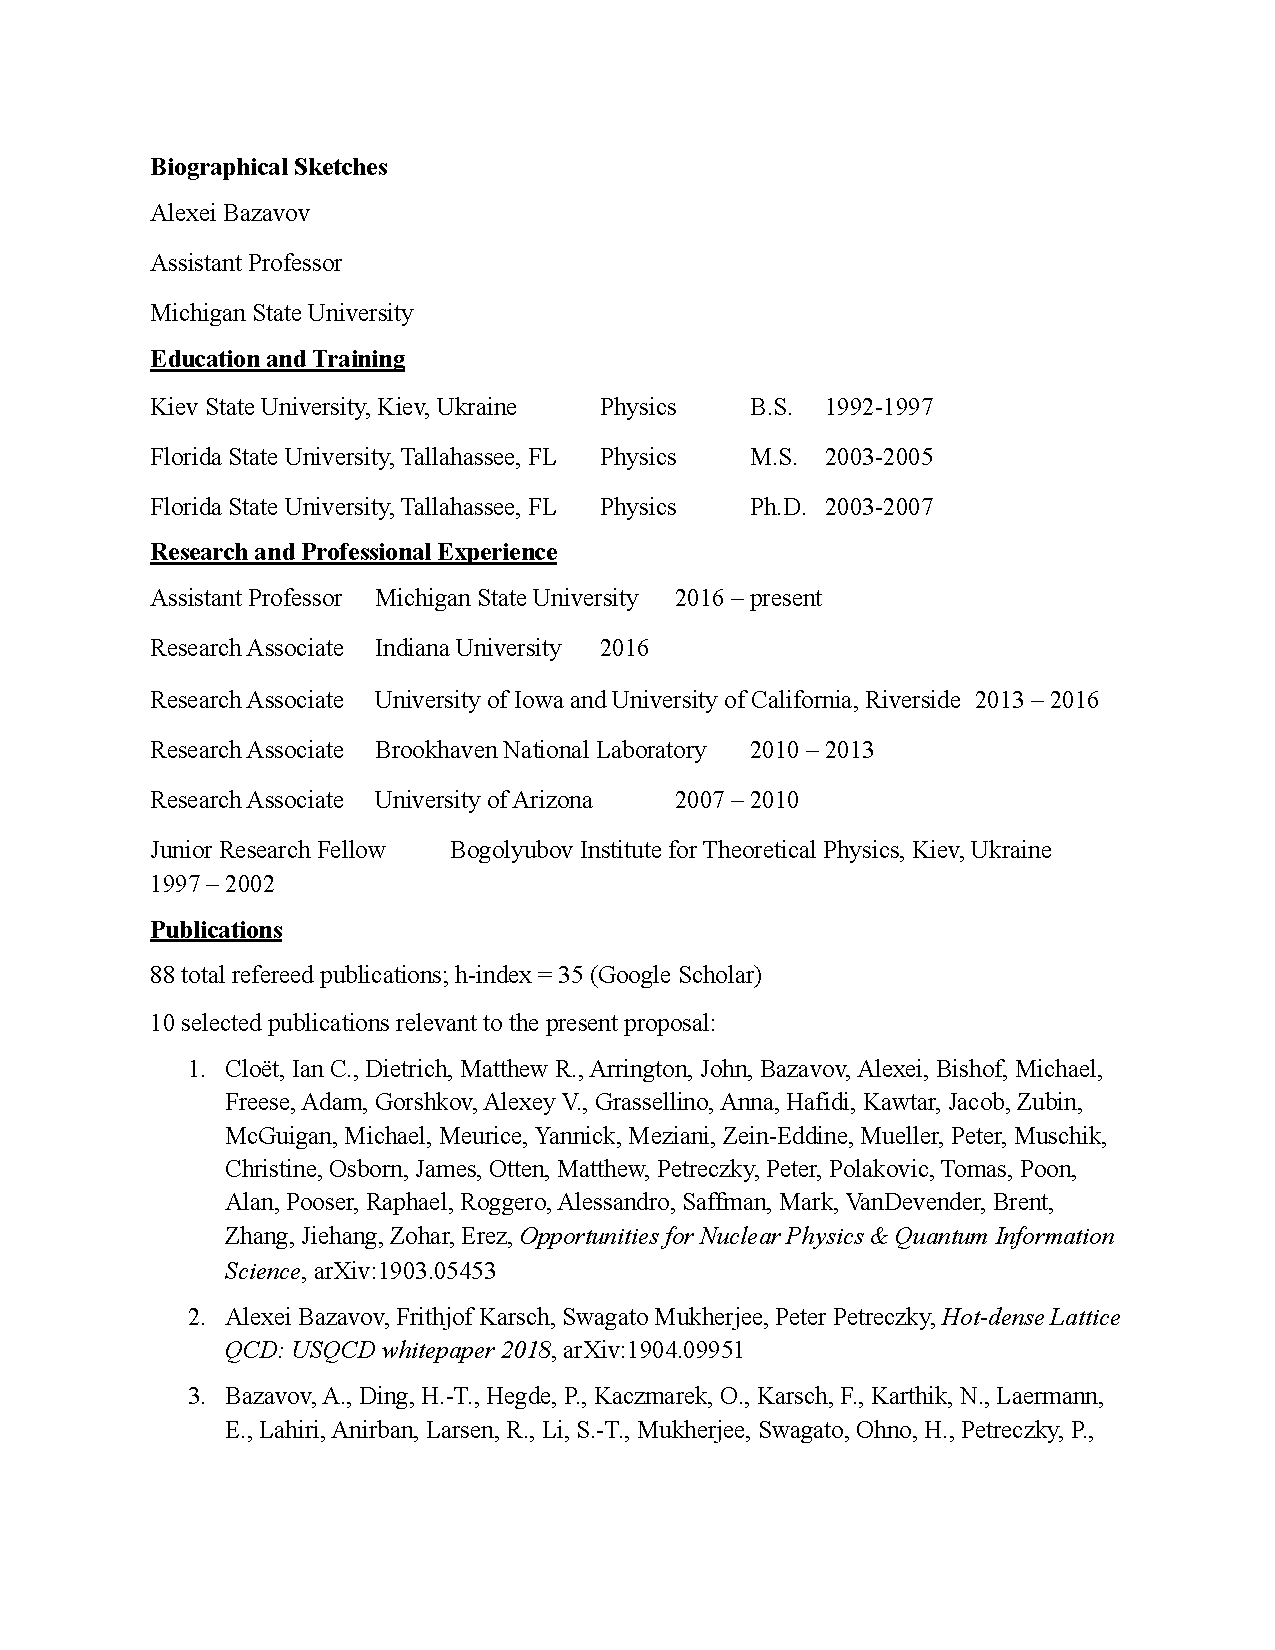
\includepdf[page=-]{bios/bio_bazavov.pdf}
\clearpage
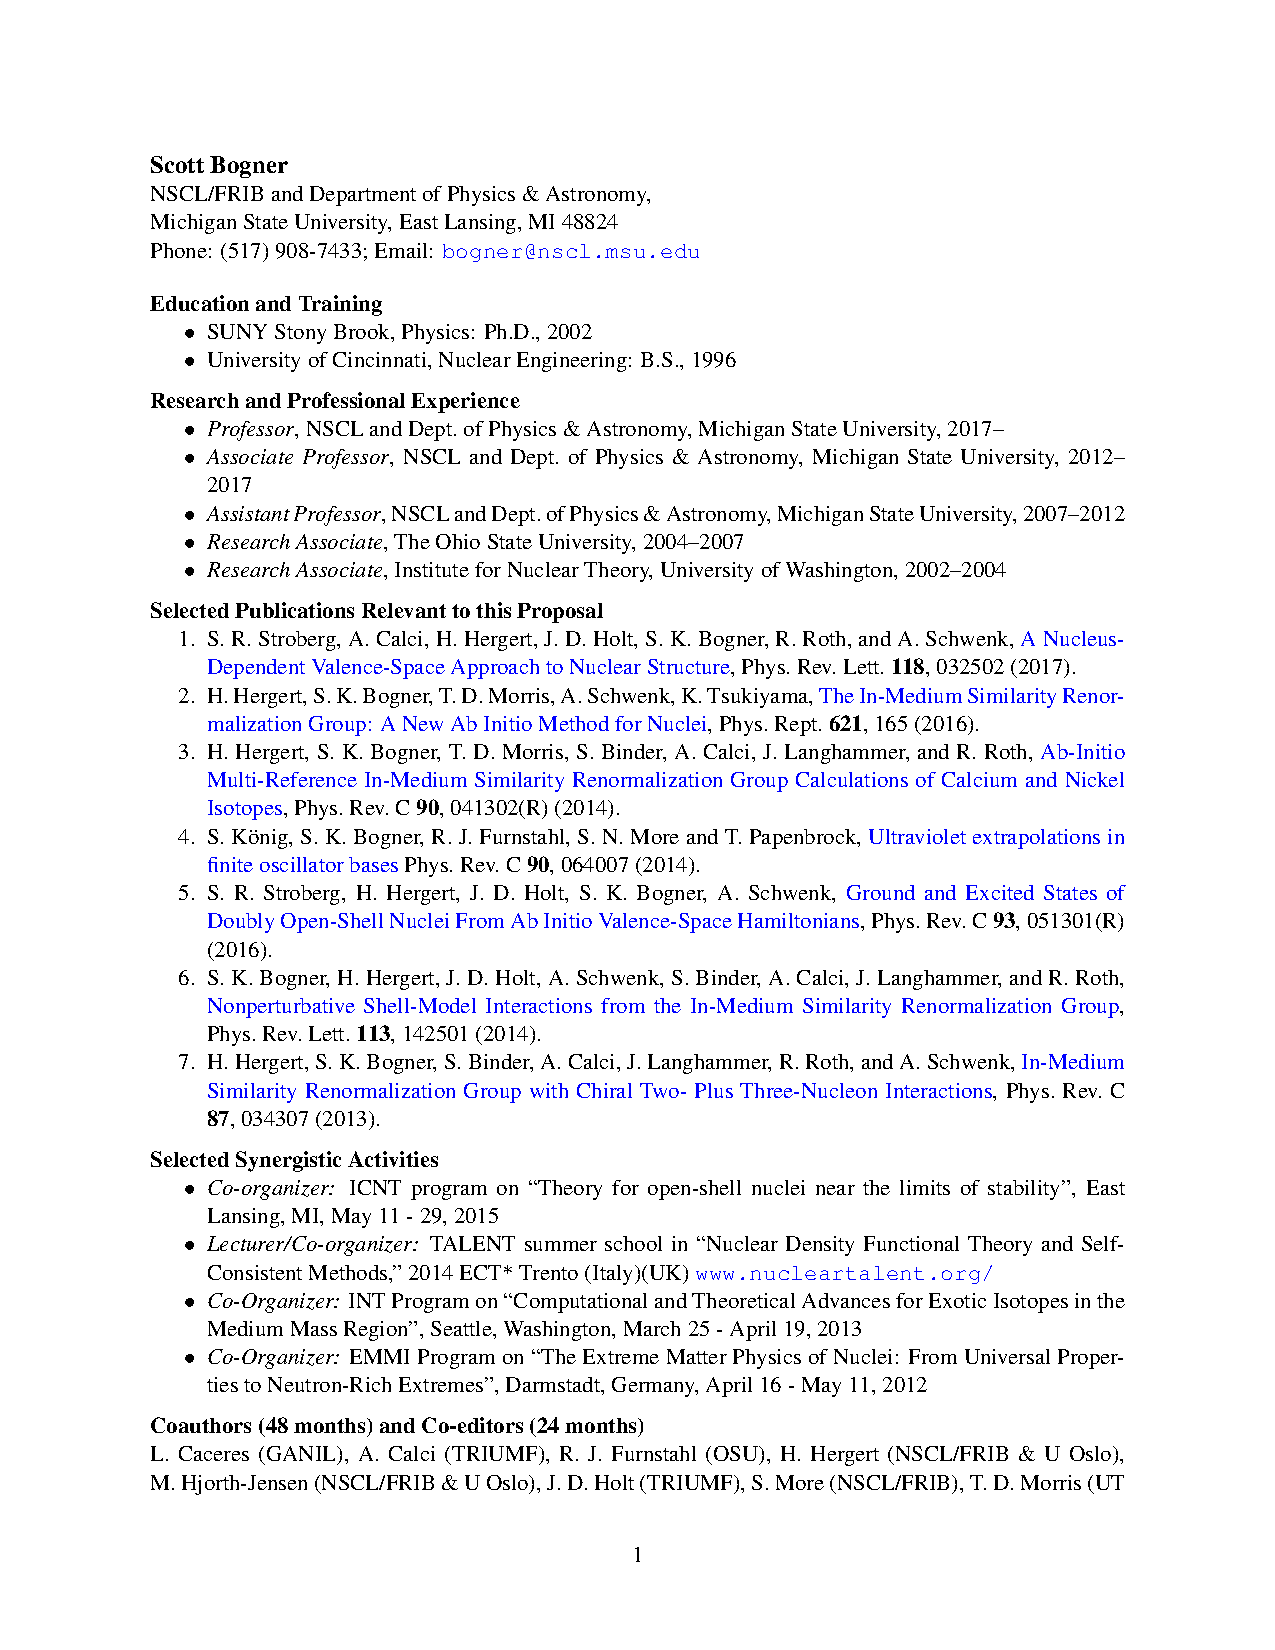
\includepdf[page=-]{bios/bio_bogner.pdf}
\clearpage
%\includepdf[page=-]{bios/bio_cosel.pdf}
\clearpage
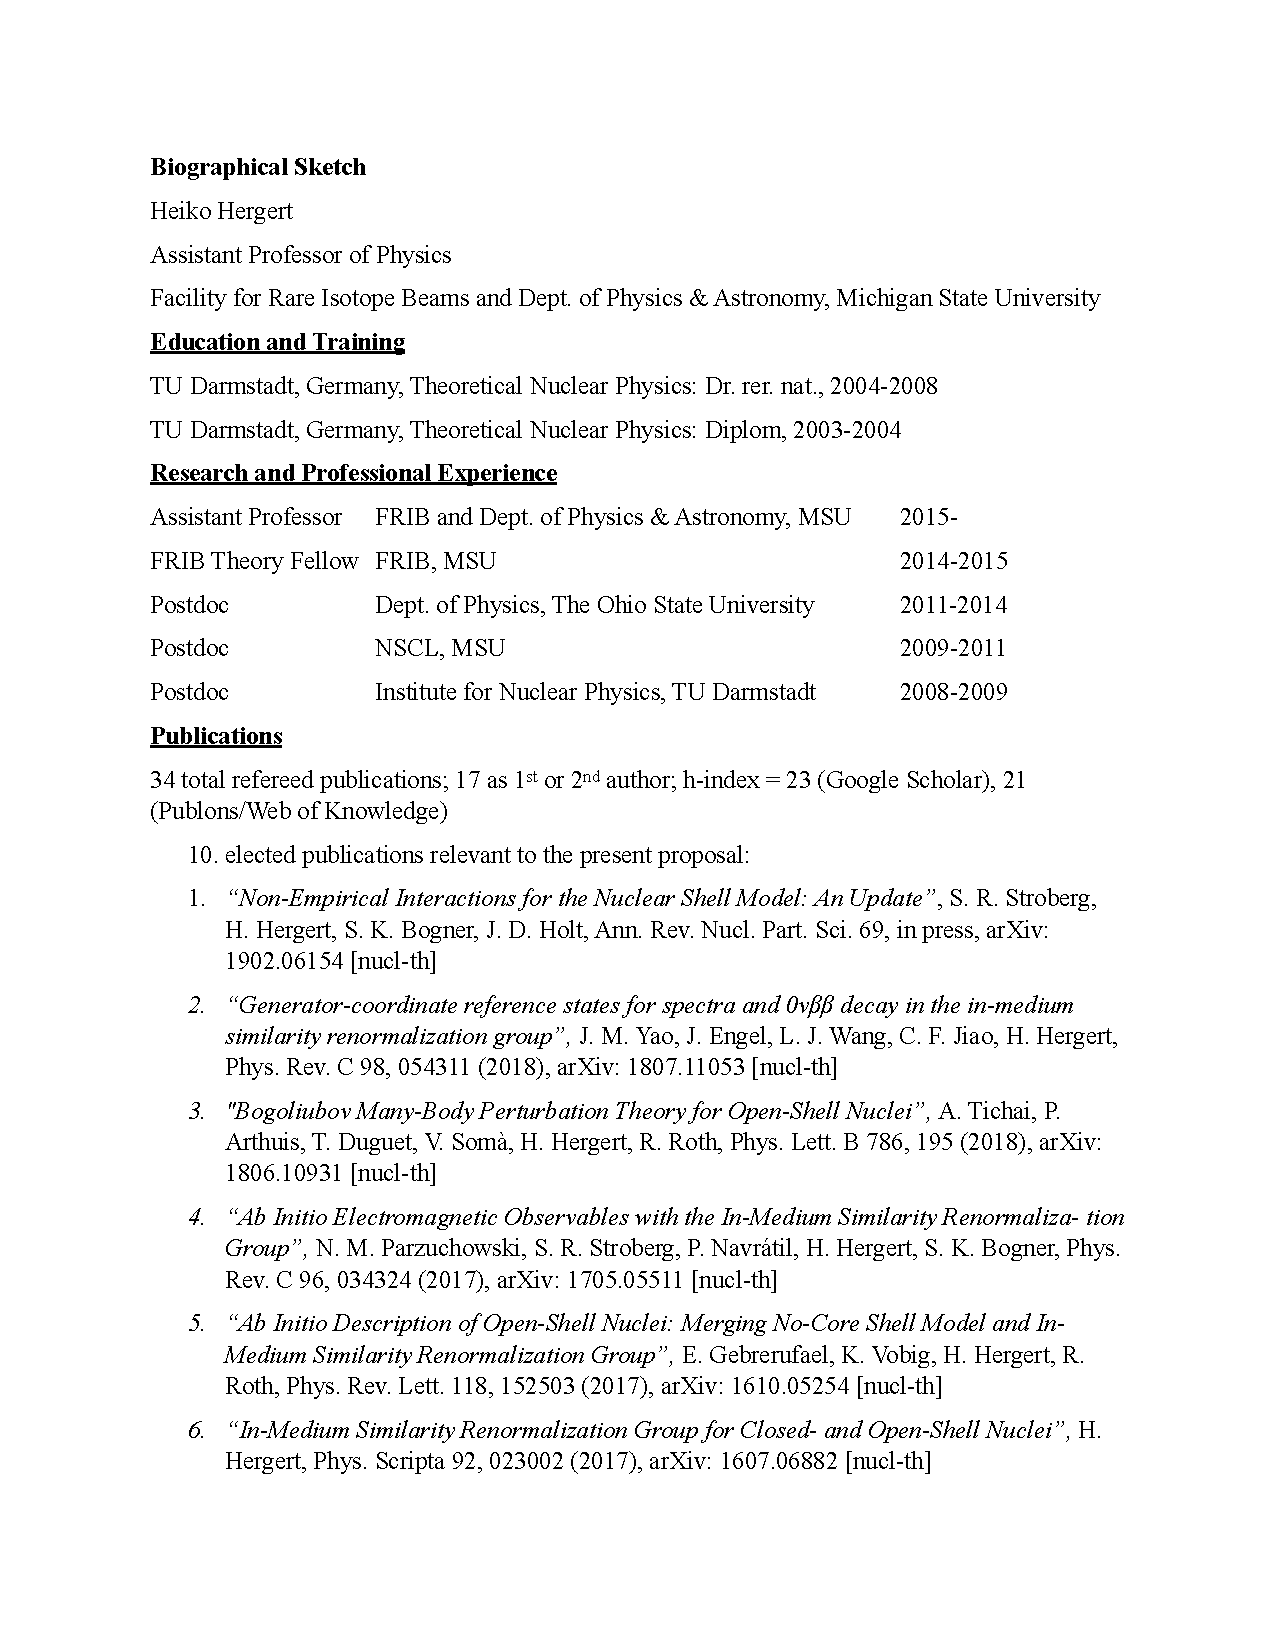
\includepdf[page=-]{bios/bio_hergert.pdf}
\clearpage
%\includepdf[page=-]{bios/bio_hirn.pdf}
\clearpage
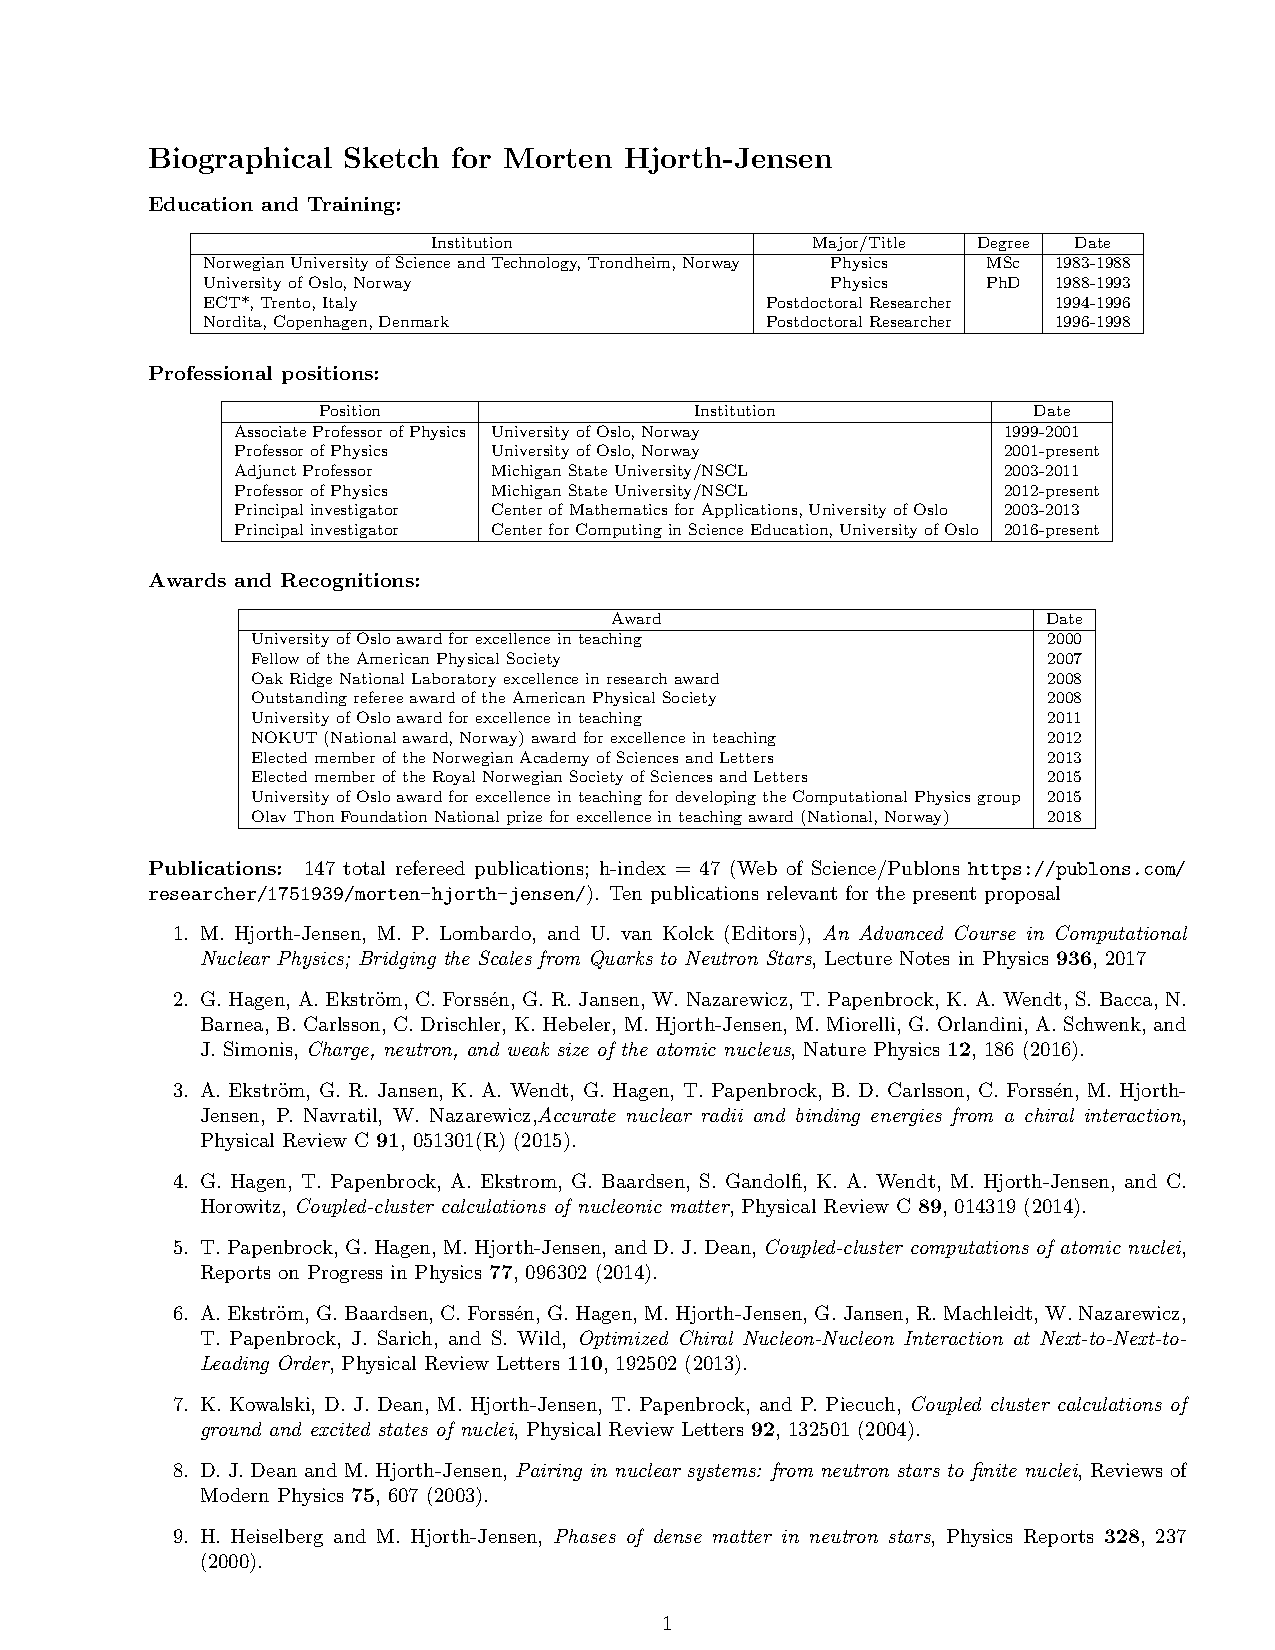
\includepdf[page=-]{bios/bio_hjorthjensen.pdf}
\clearpage
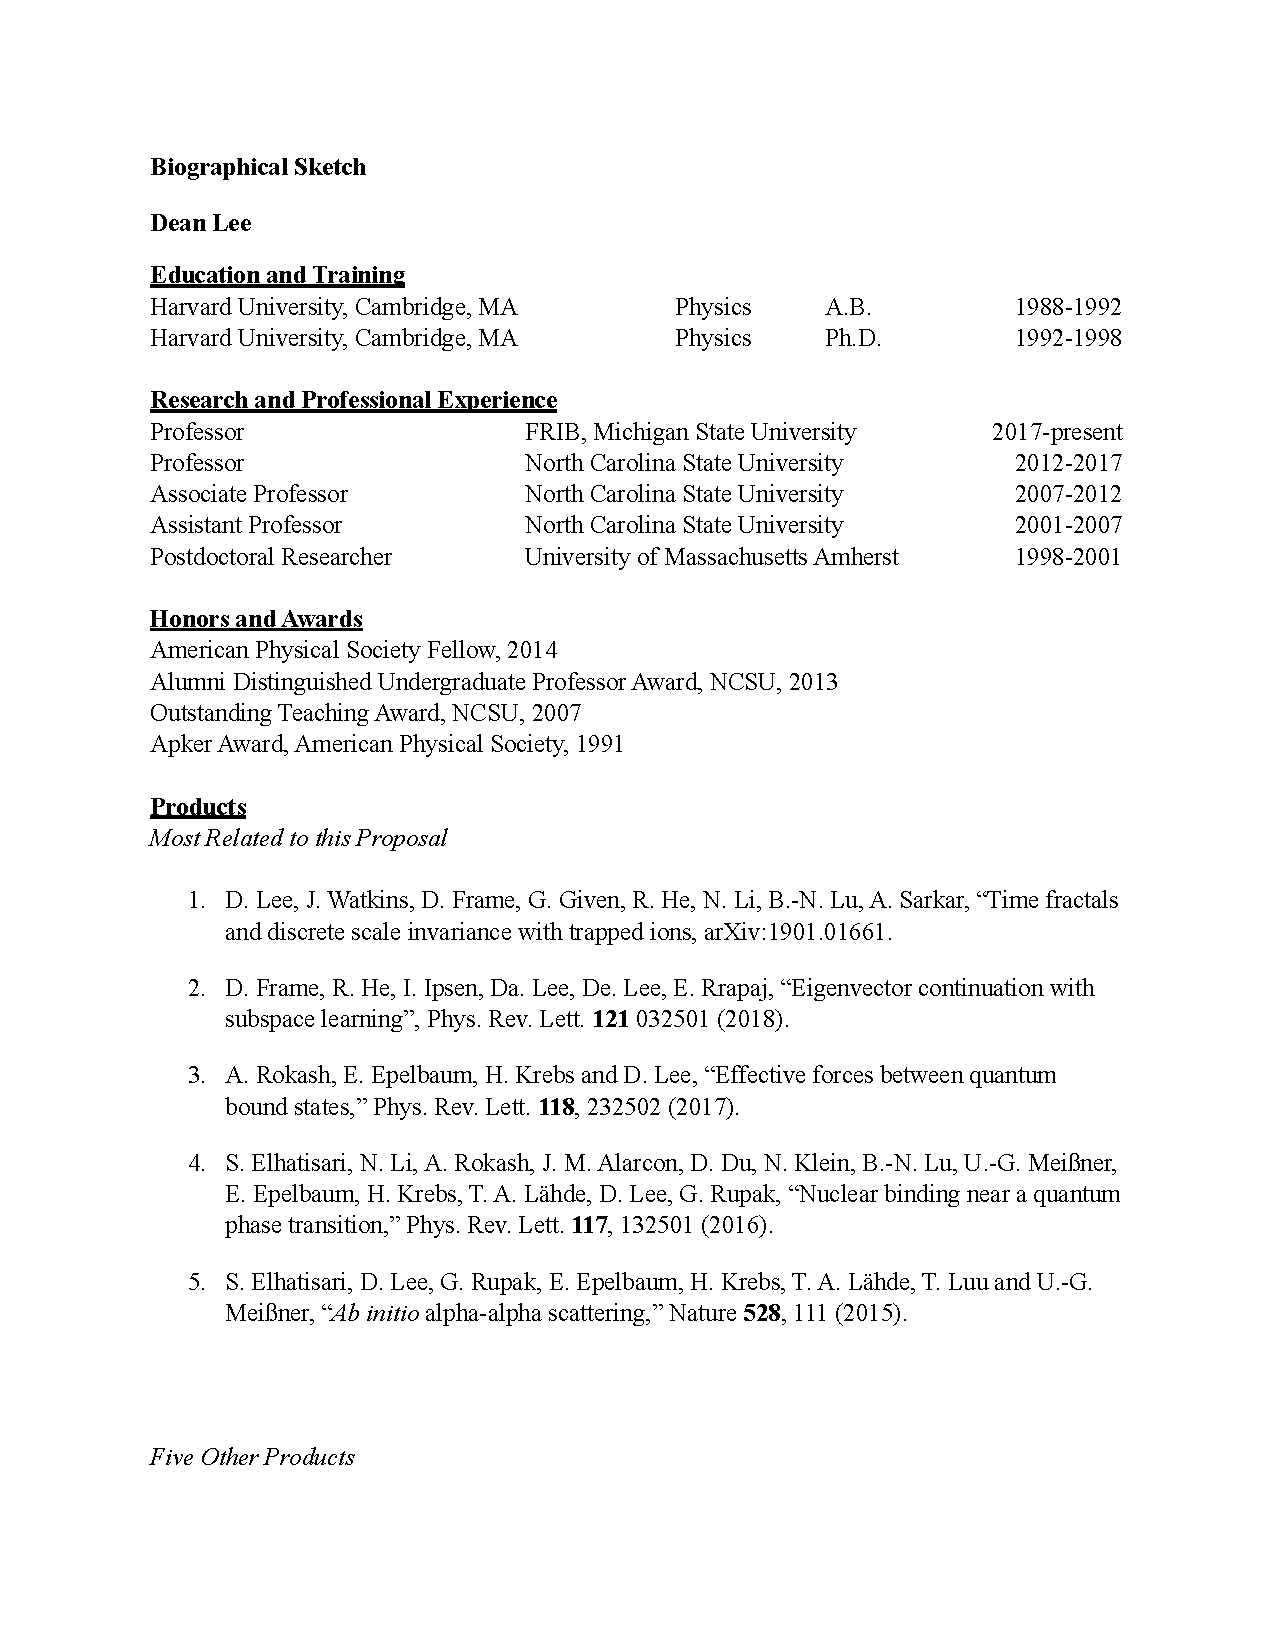
\includepdf[page=-]{bios/bio_lee.pdf}
\clearpage
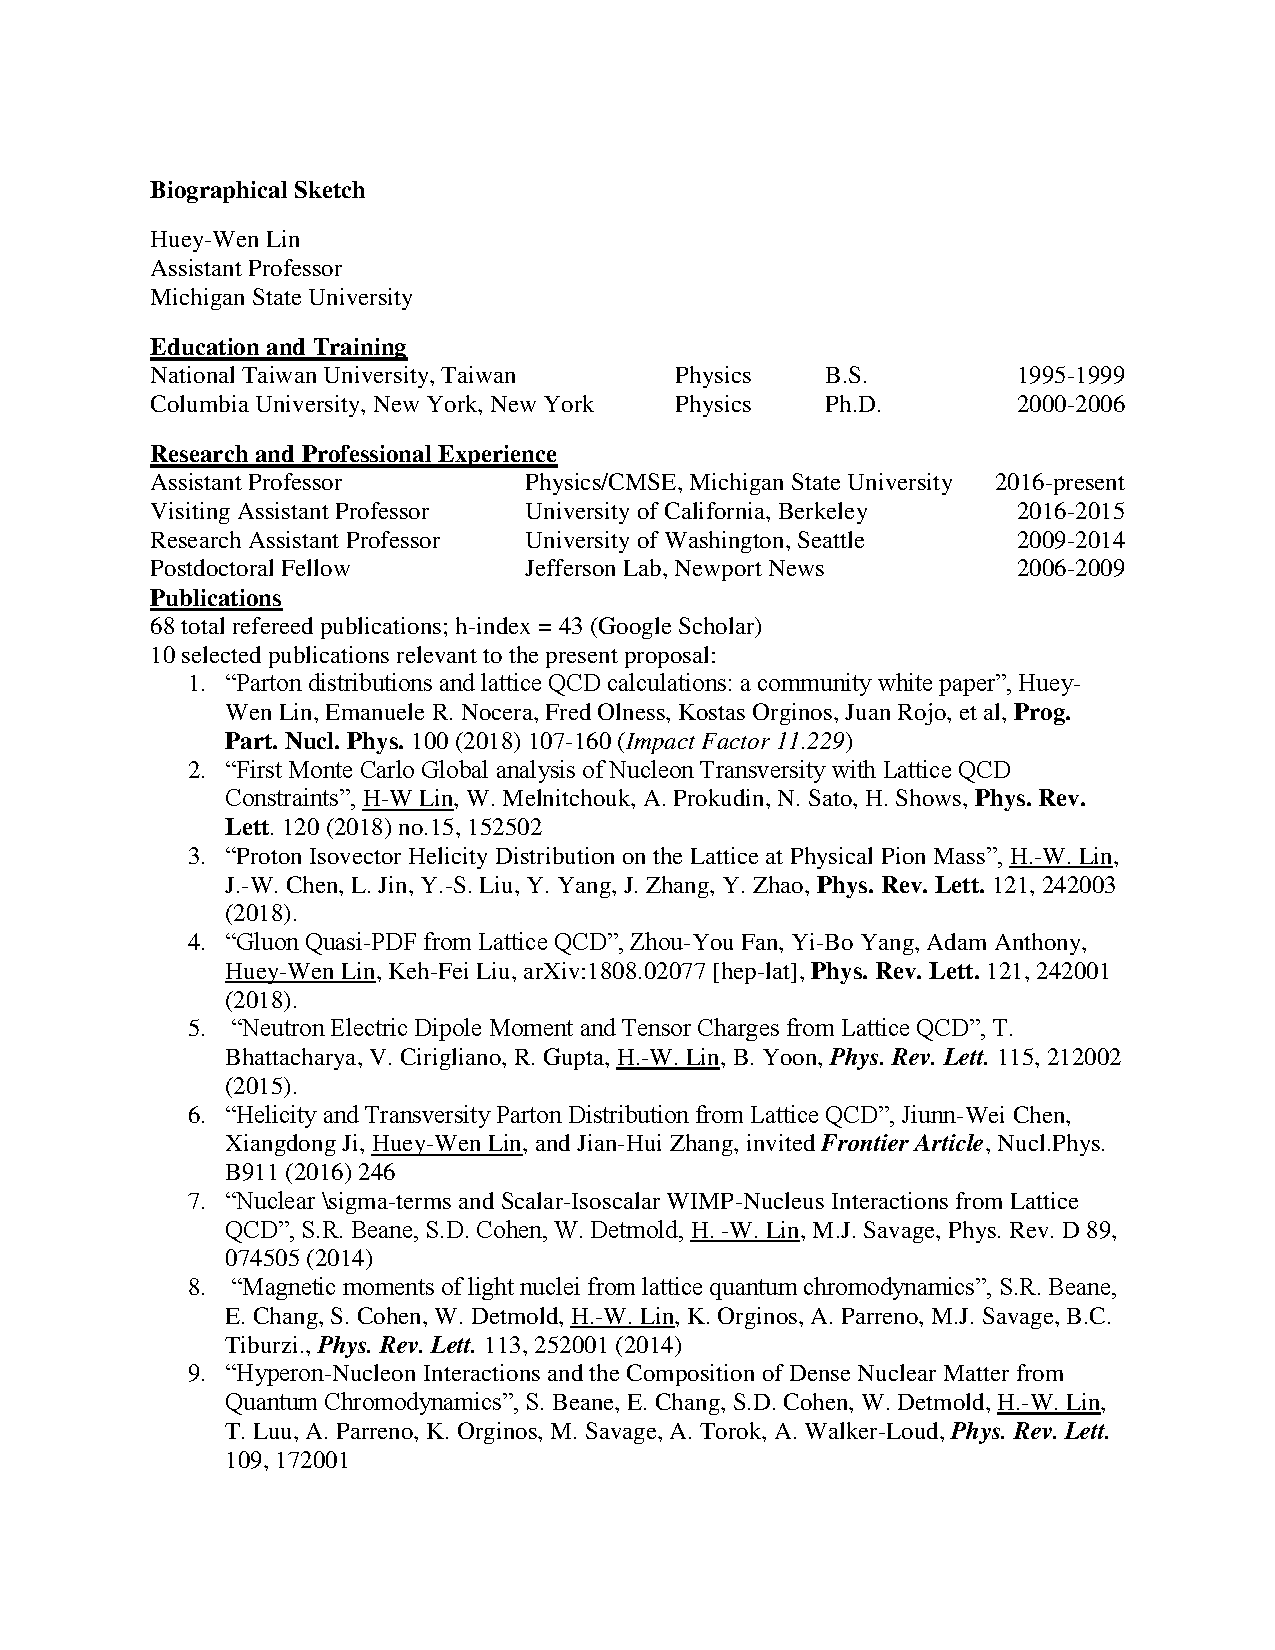
\includepdf[page=-]{bios/bio_lin.pdf}
\clearpage
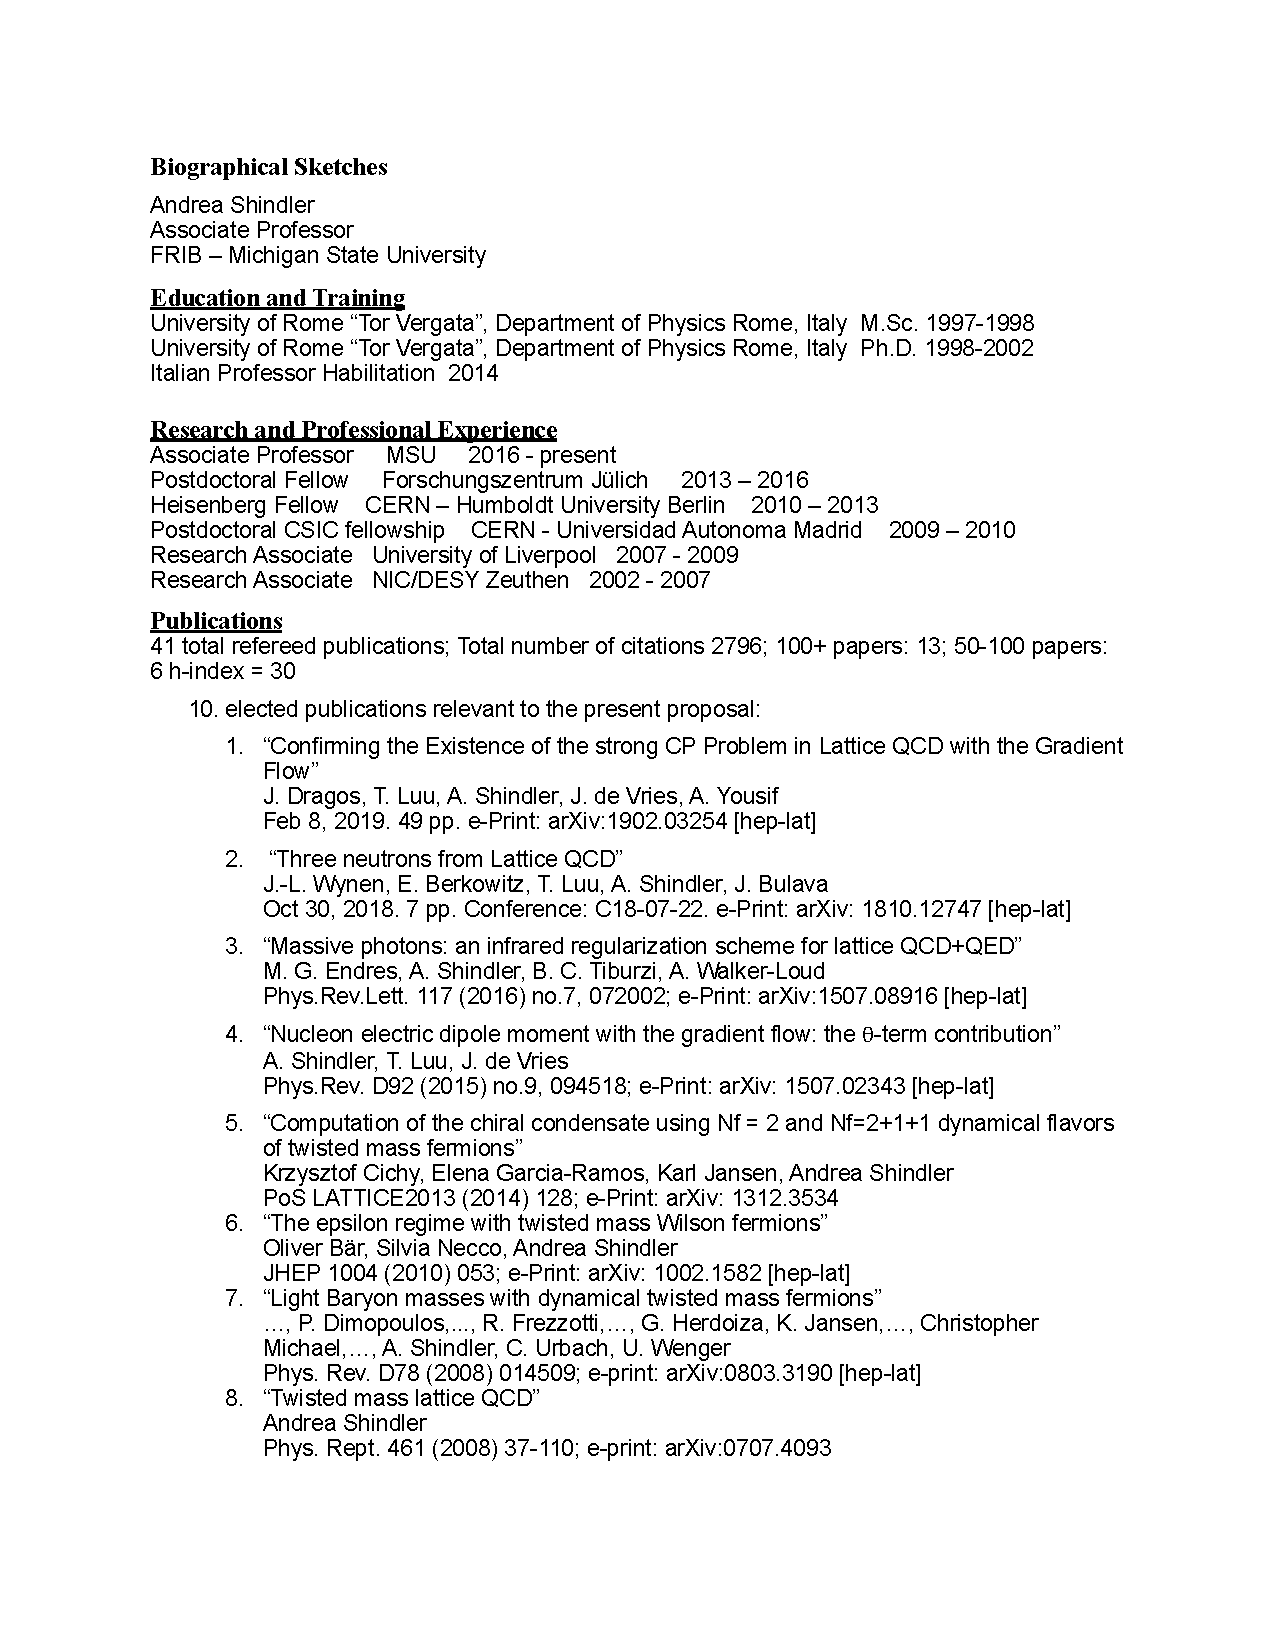
\includepdf[page=-]{bios/bio_shindler.pdf}
\clearpage
\section{Current and Pending Support}

Current and pending support of the senior personnel follow in alphabetical order.
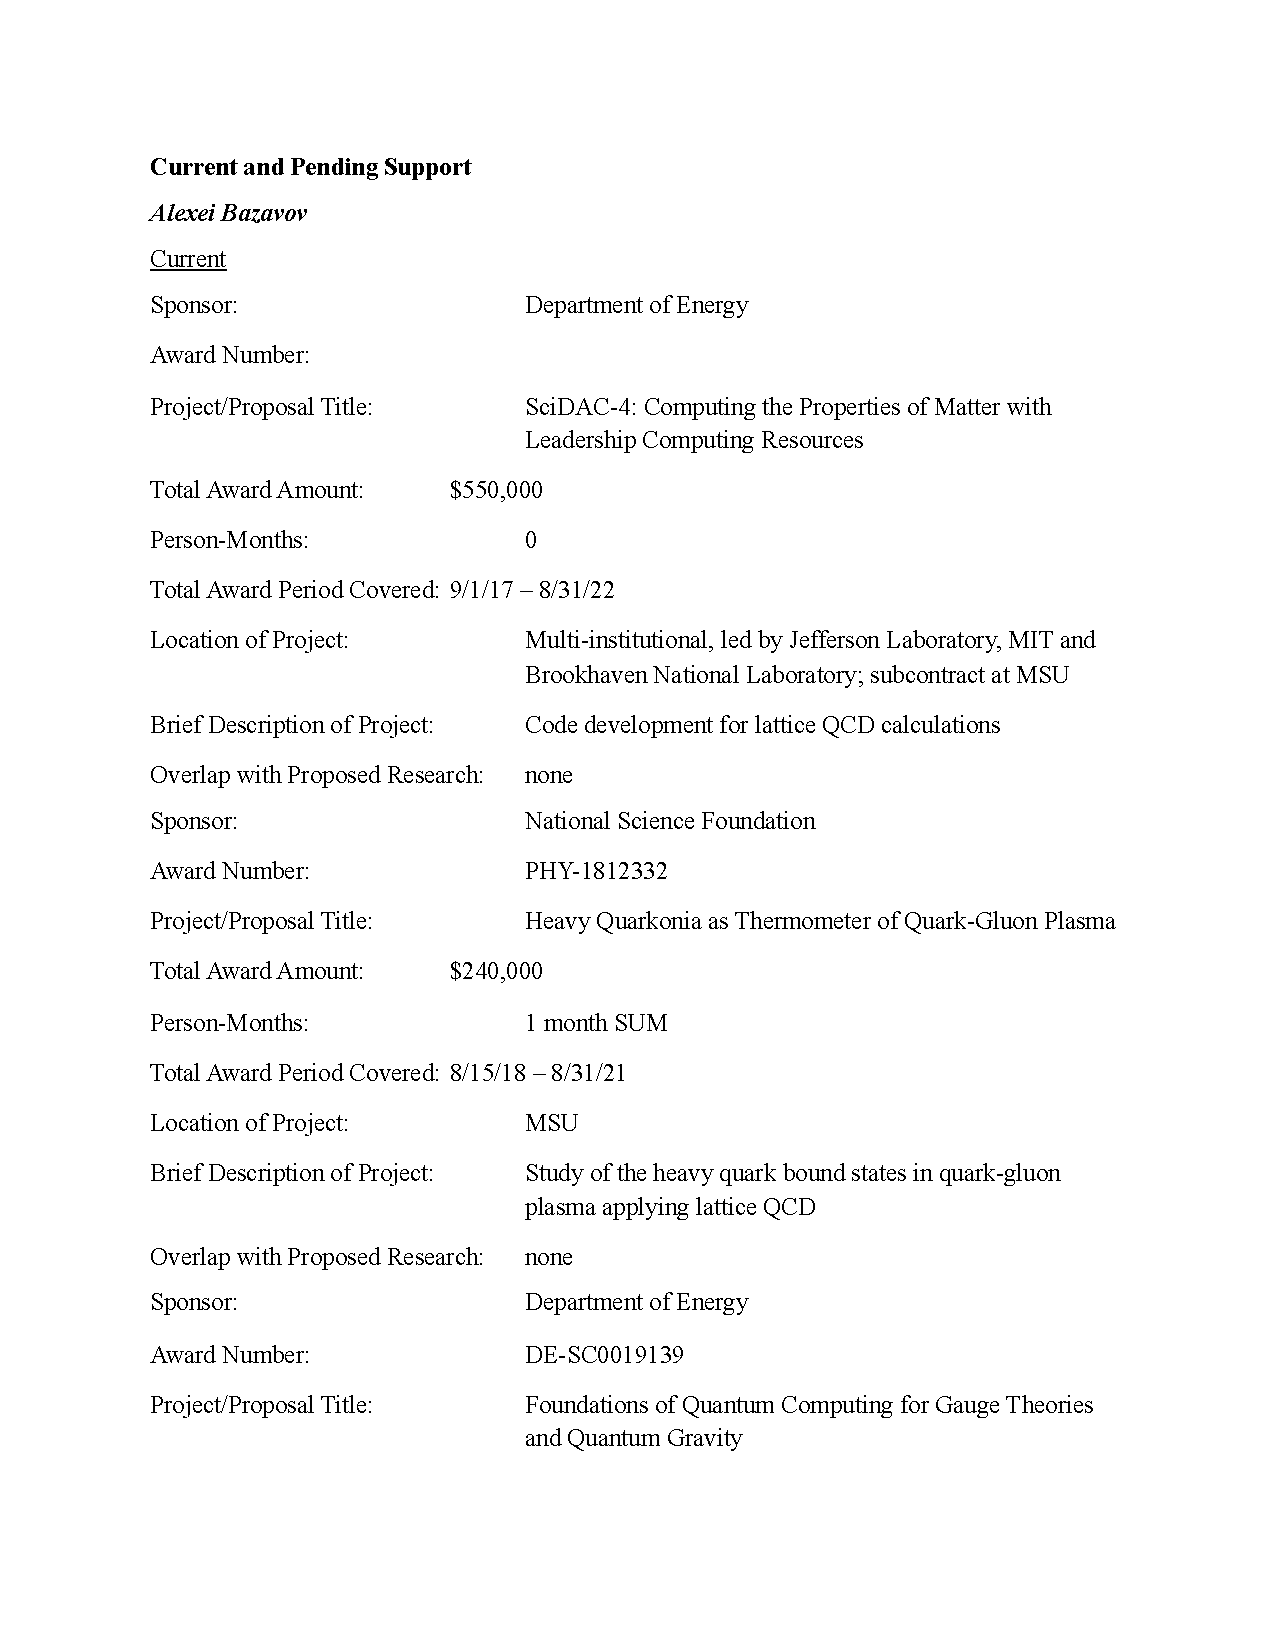
\includepdf[page=-]{support/support_bazavov.pdf}
\clearpage
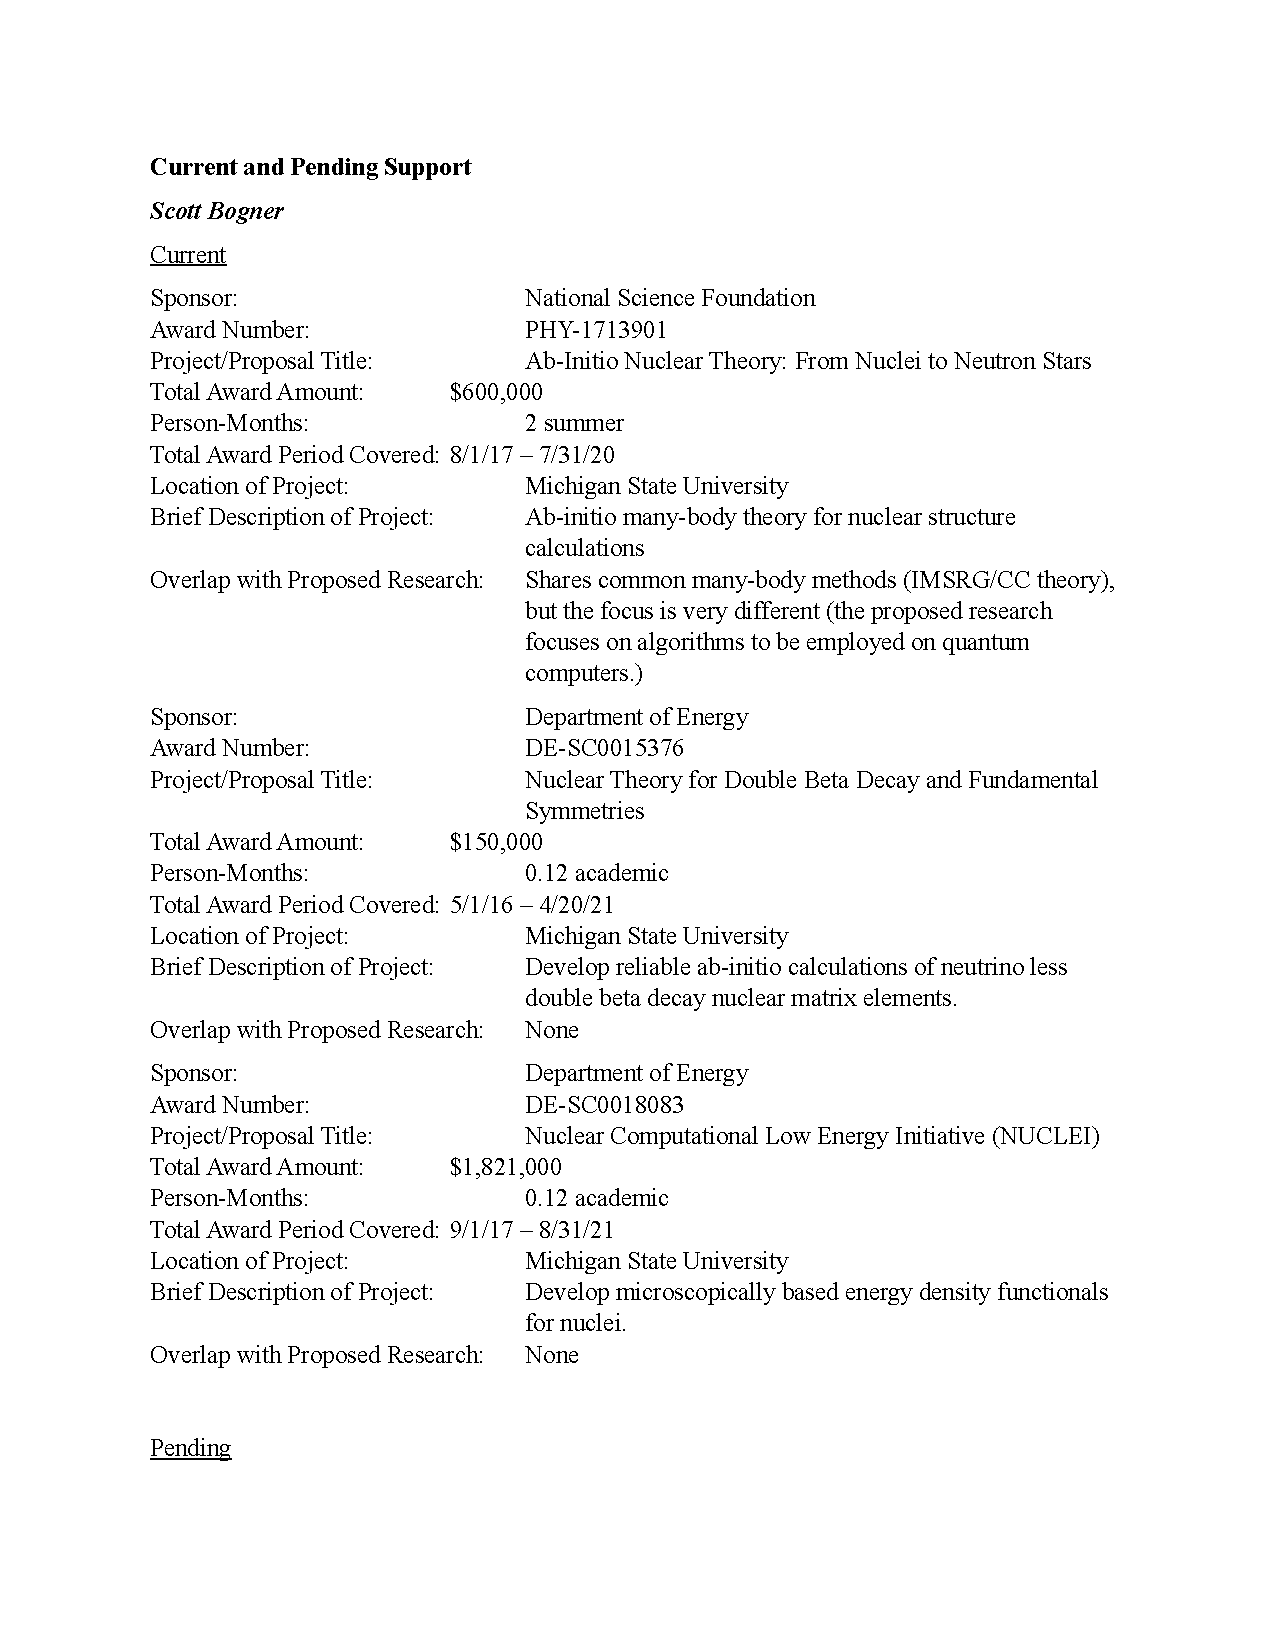
\includepdf[page=-]{support/support_bogner.pdf}
\clearpage
%\includepdf[page=-]{support/support_cosel.pdf}
\clearpage
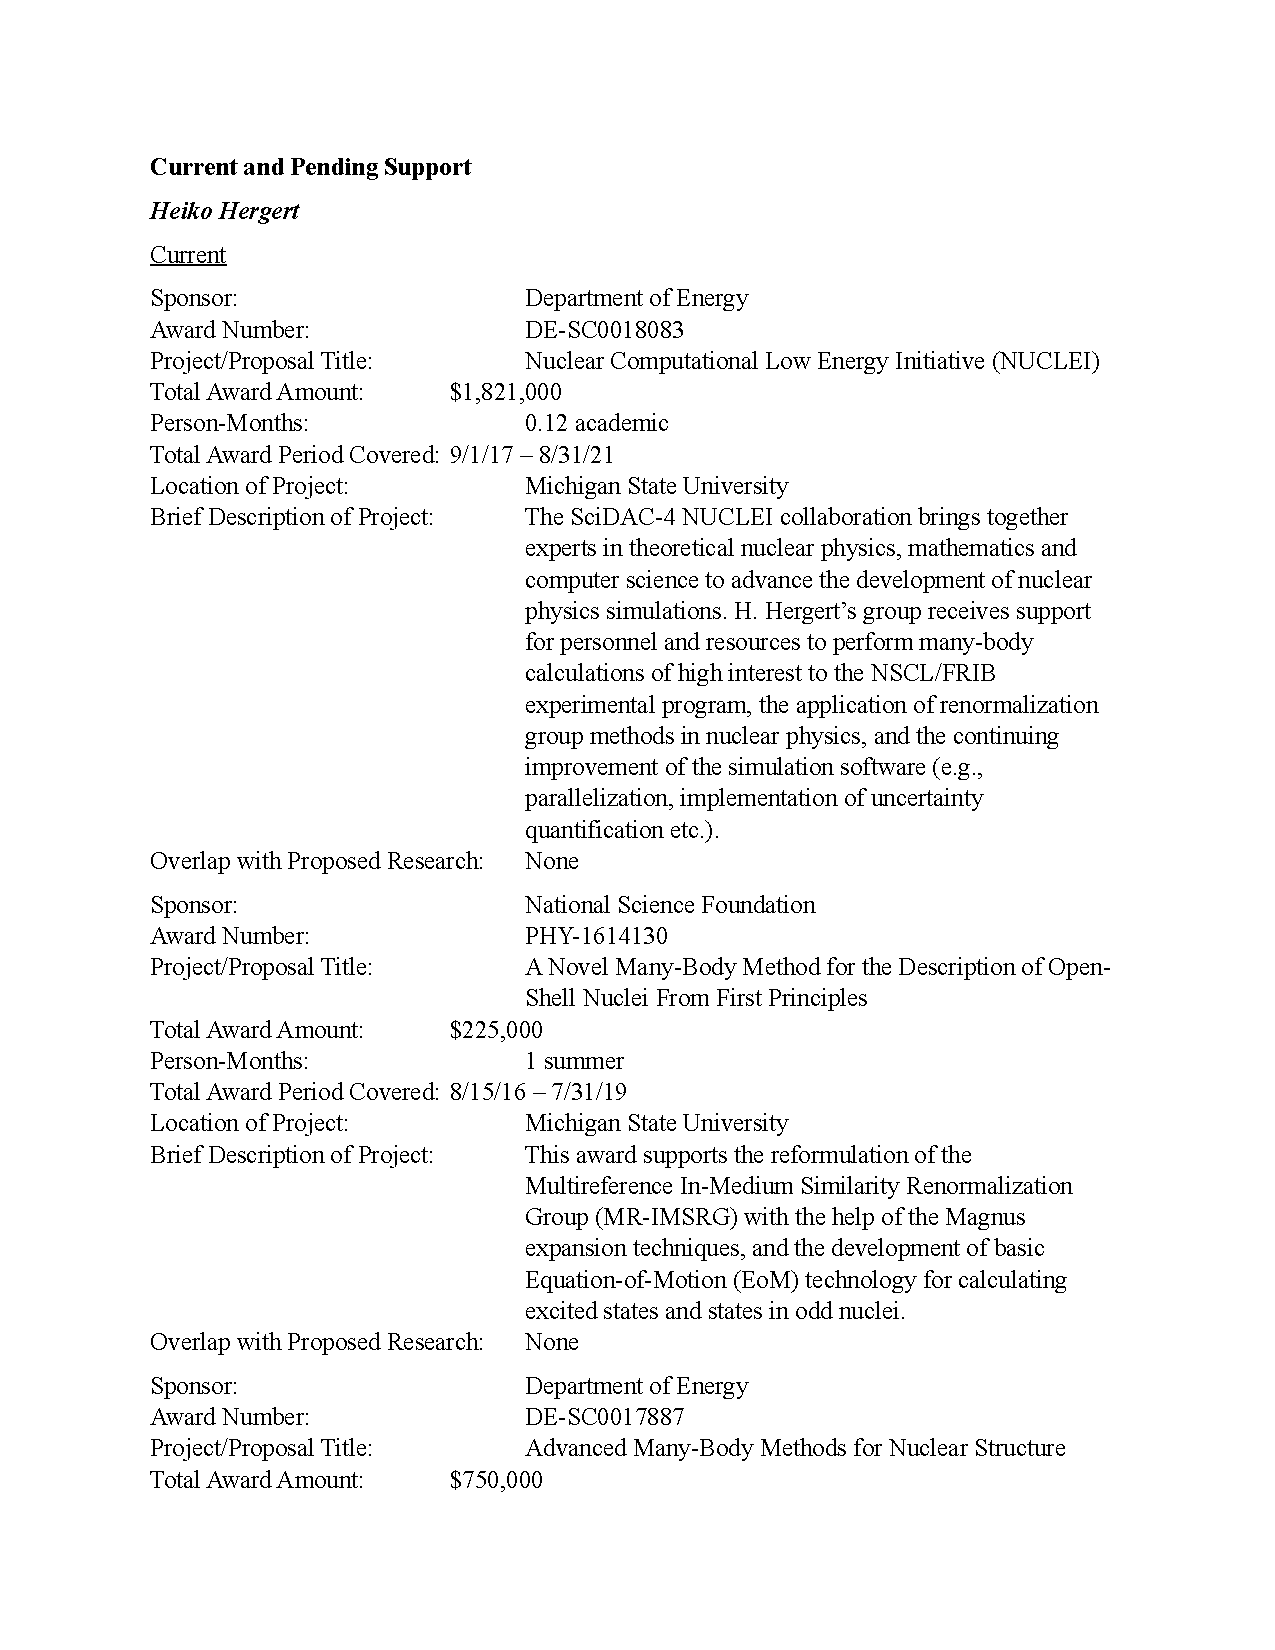
\includepdf[page=-]{support/support_hergert.pdf}
\clearpage
%\includepdf[page=-]{support/support_hirn.pdf}
\clearpage
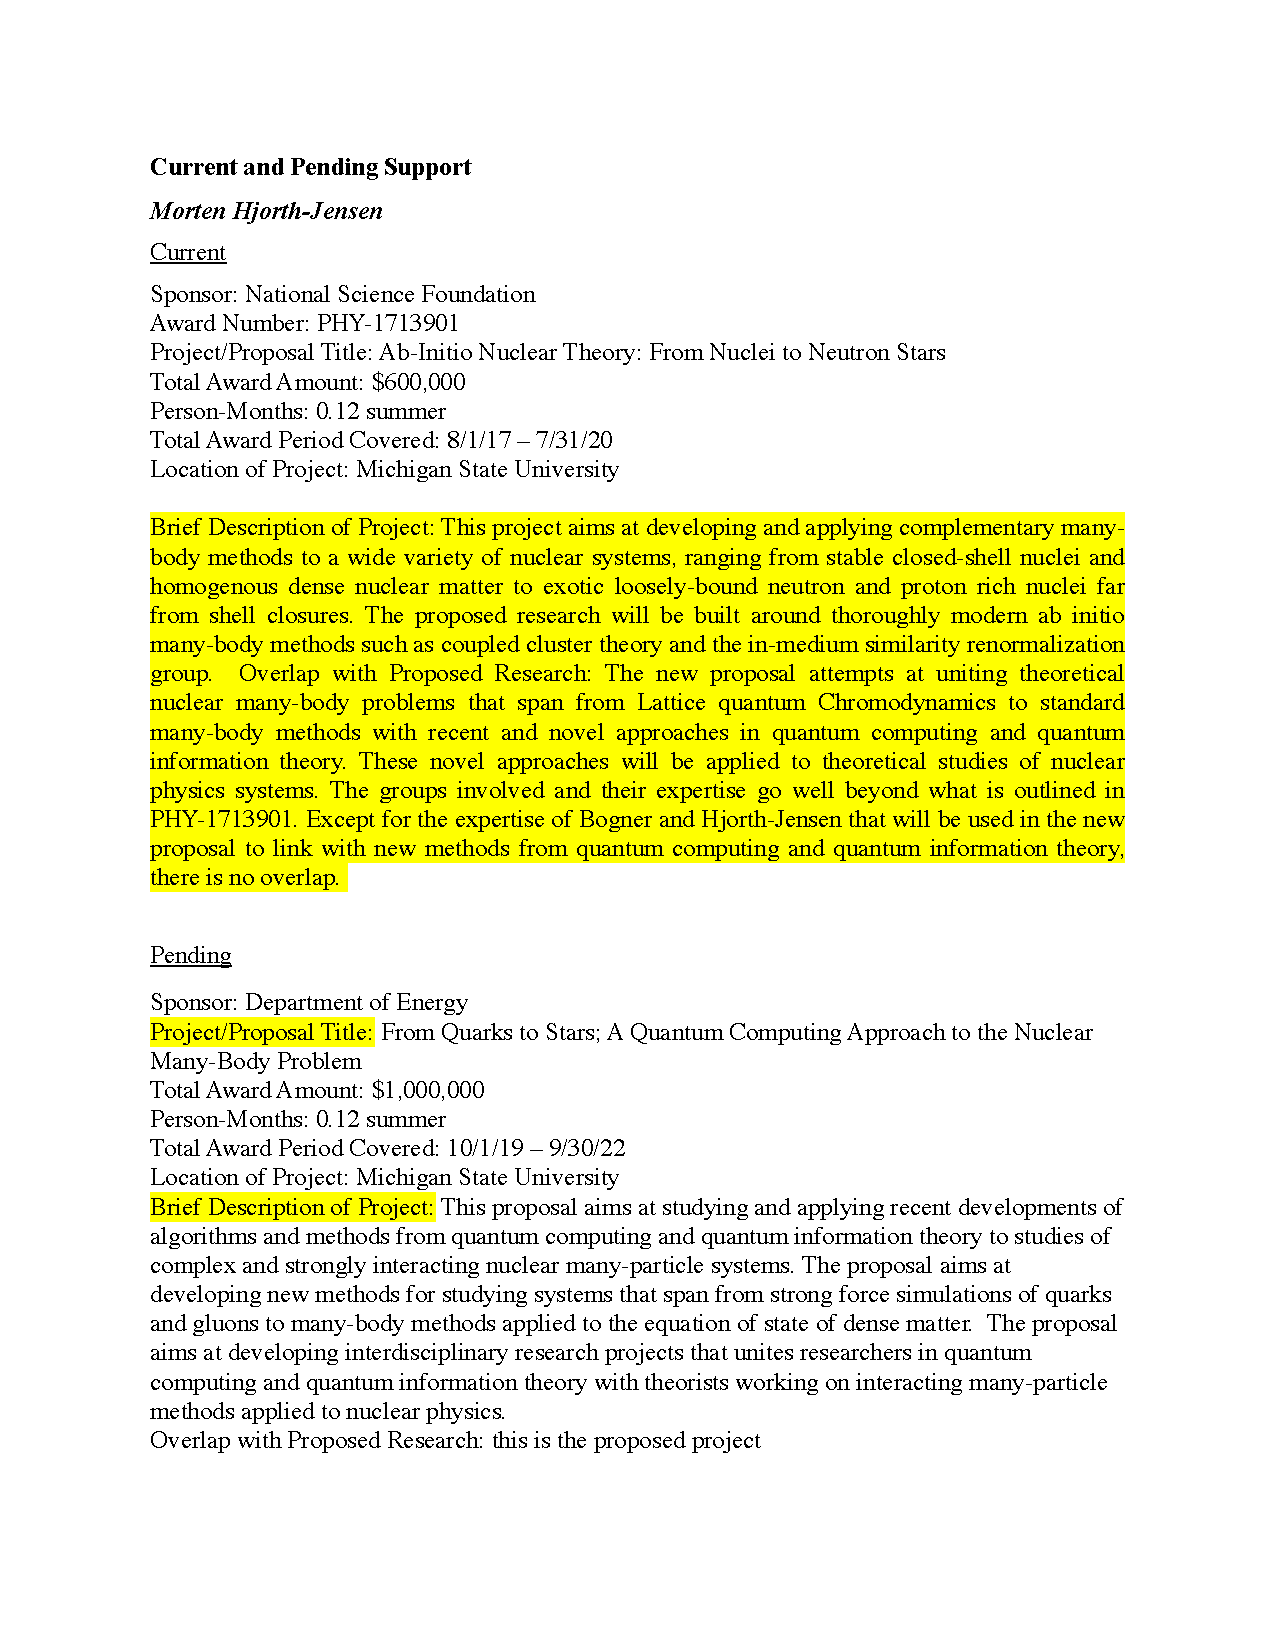
\includepdf[page=-]{support/support_hjorthjensen.pdf}
\clearpage
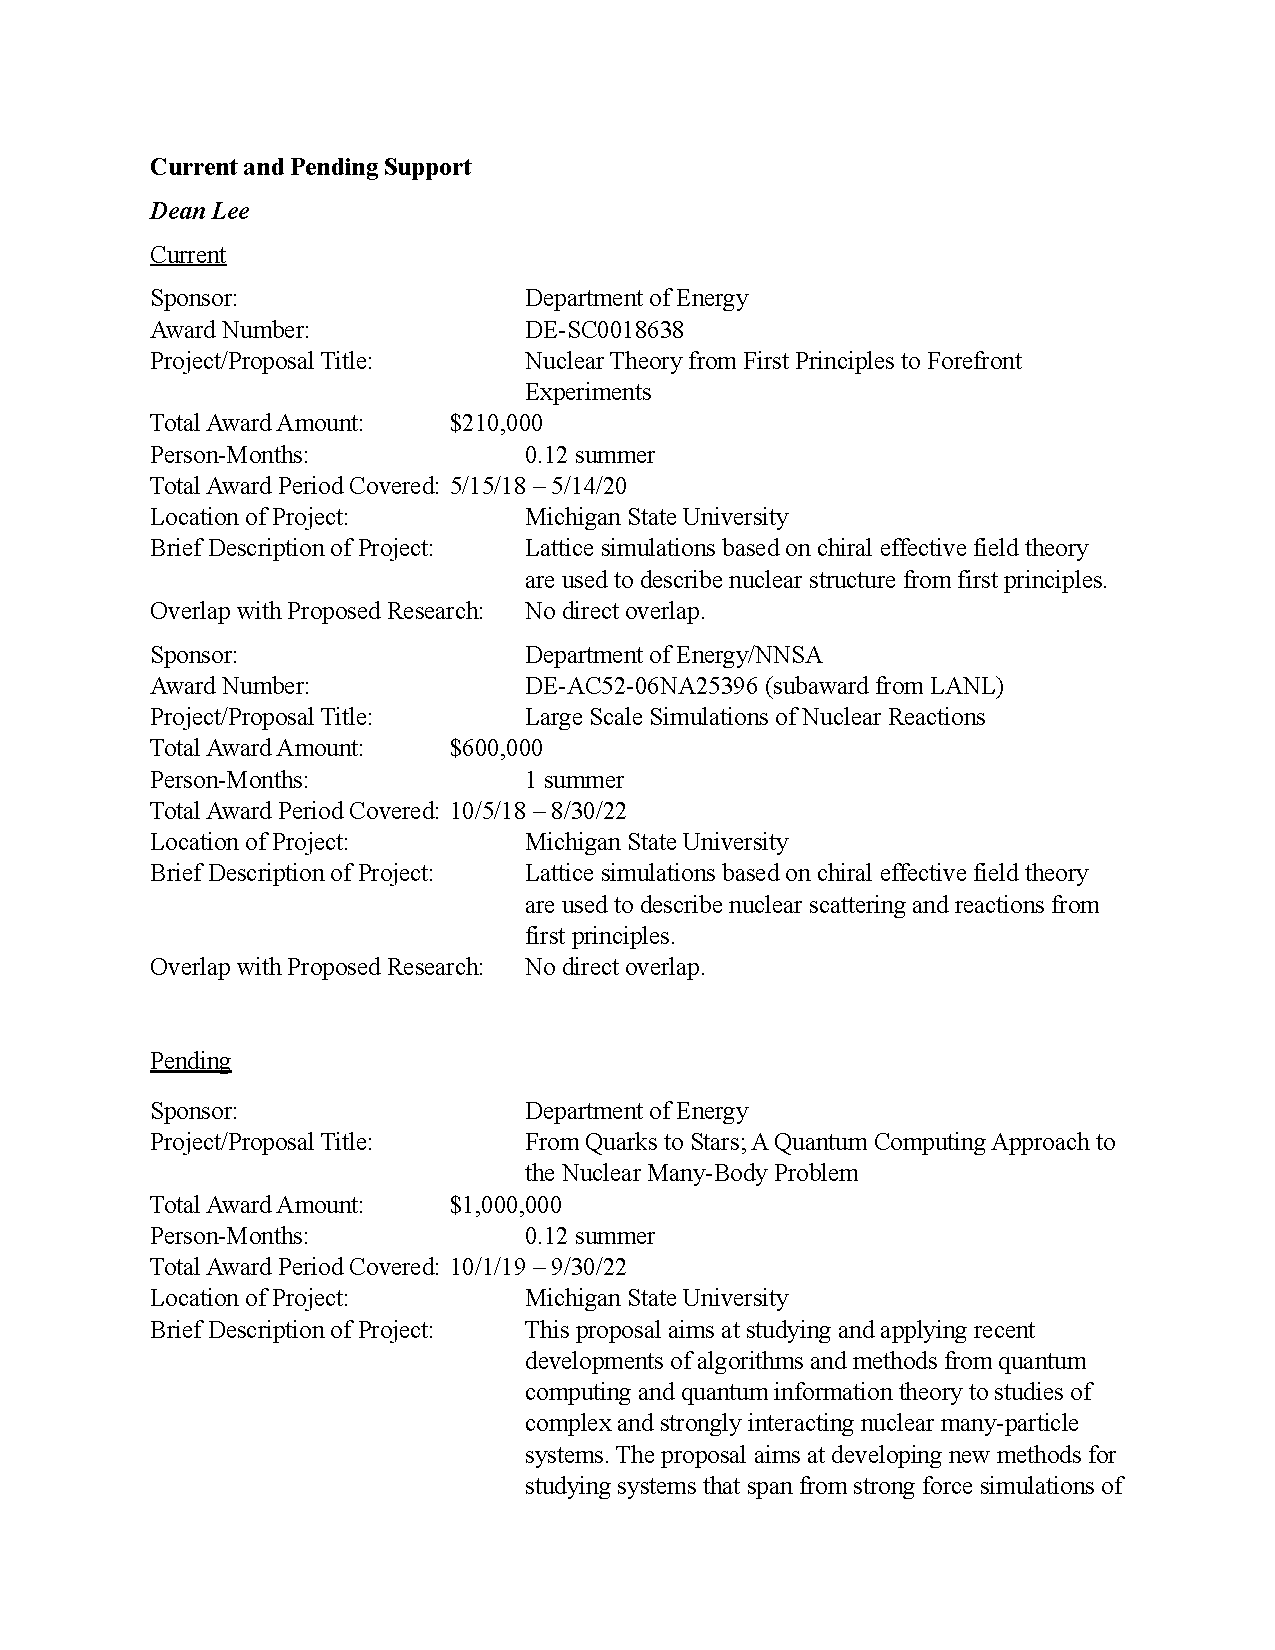
\includepdf[page=-]{support/support_lee.pdf}
\clearpage
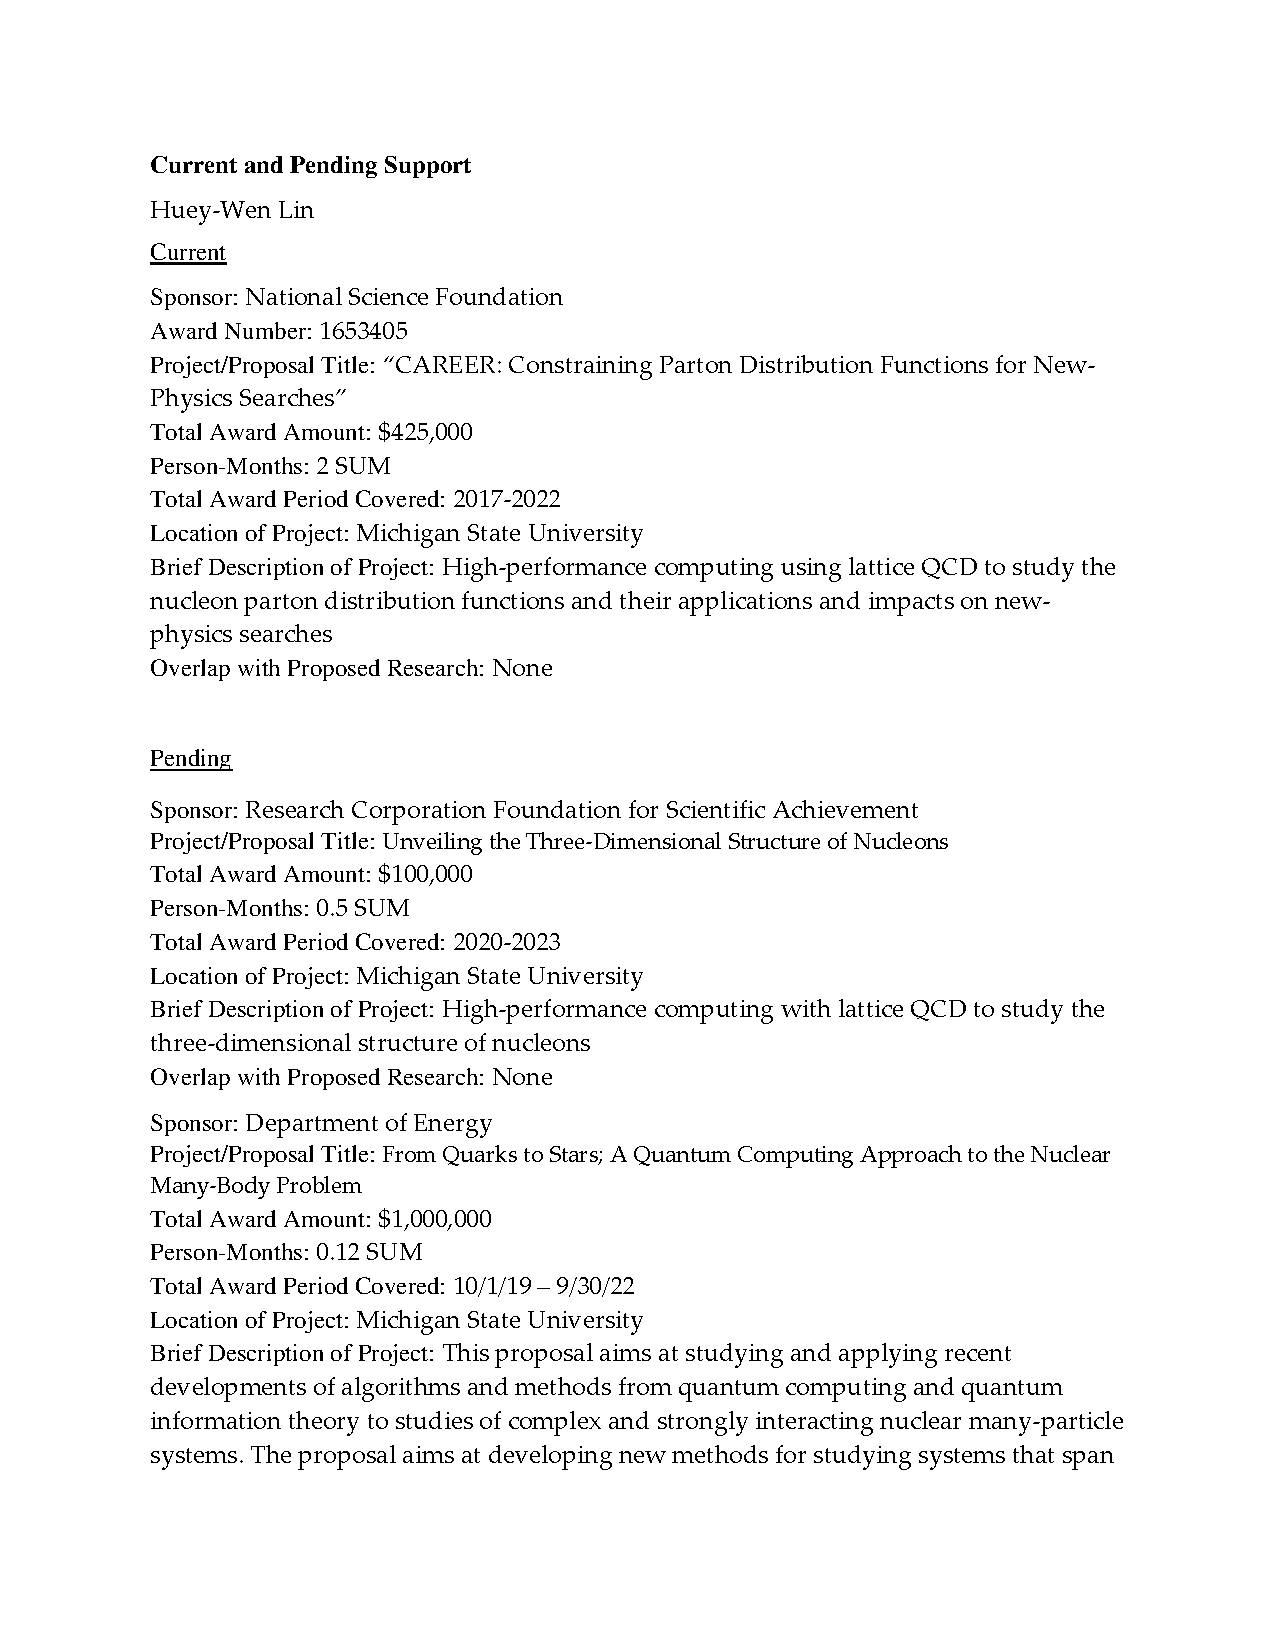
\includepdf[page=-]{support/support_lin.pdf}
\clearpage
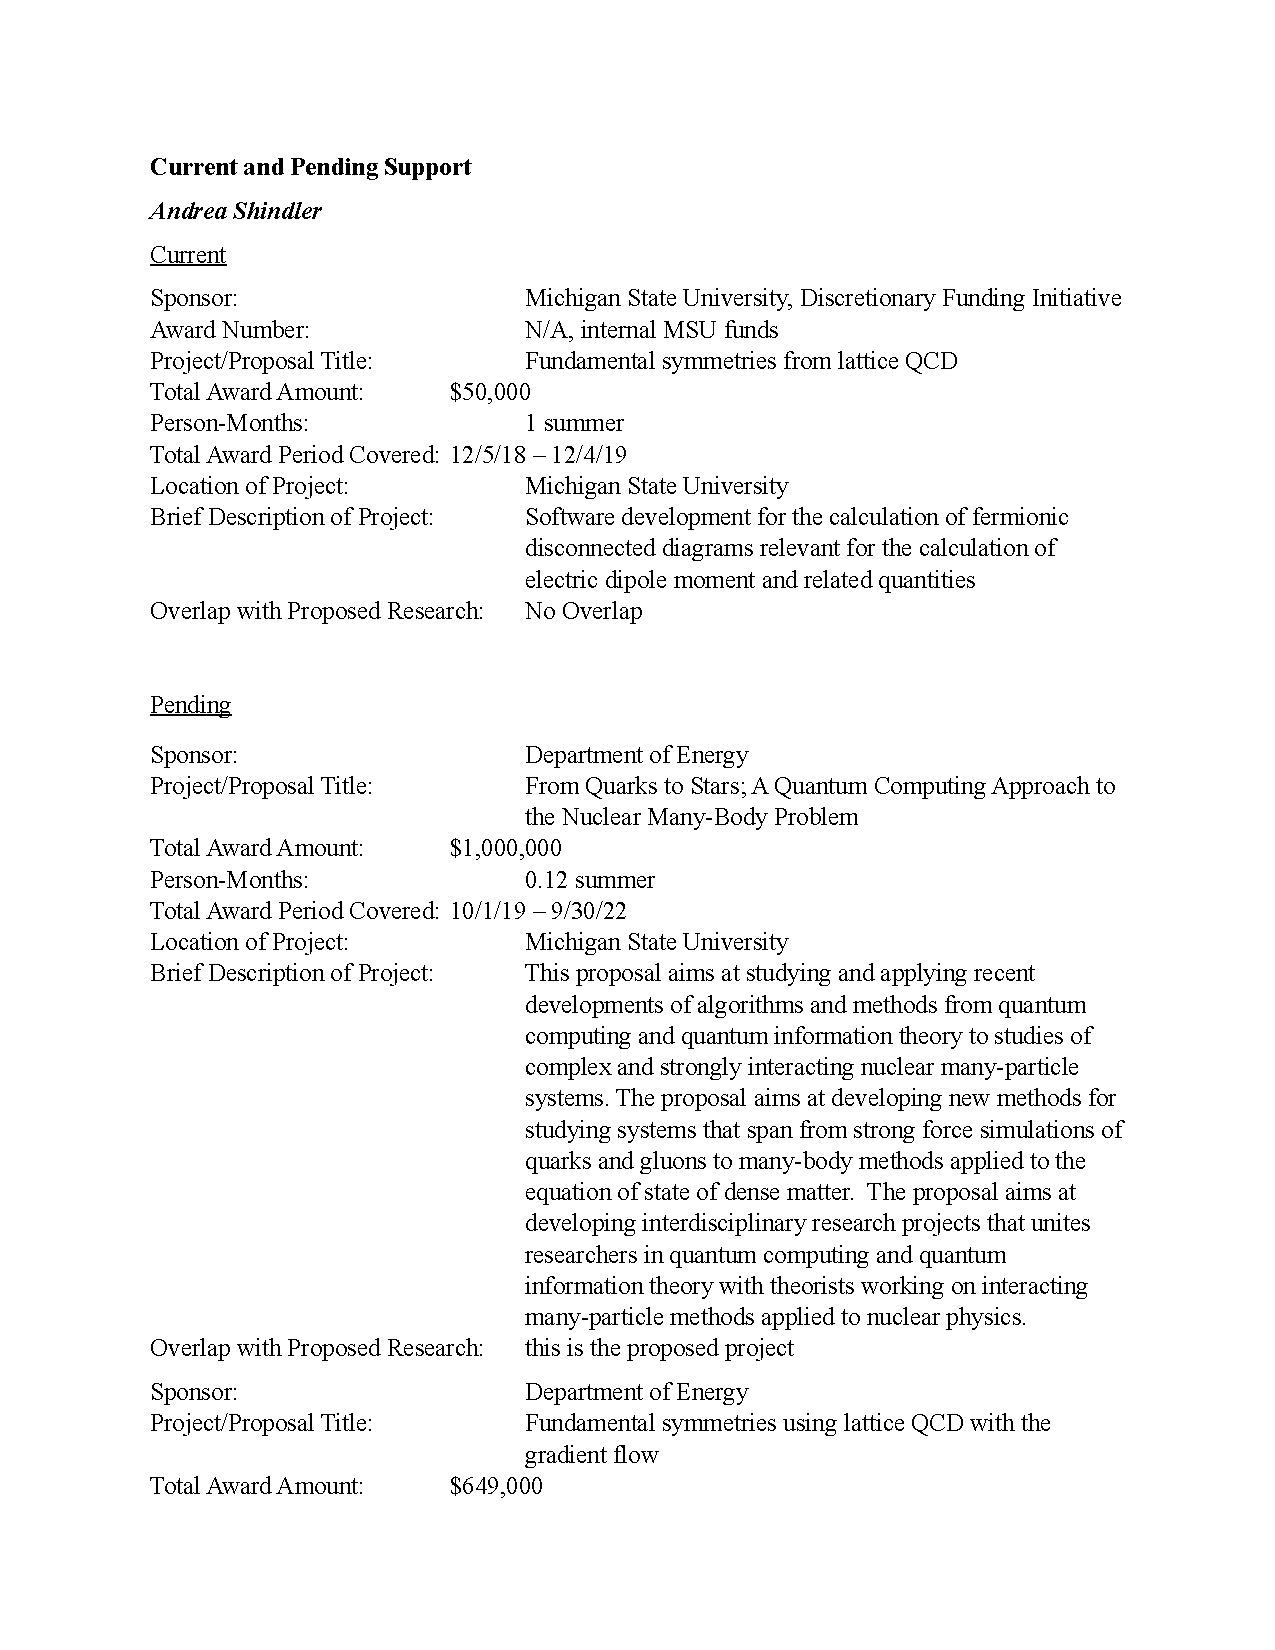
\includepdf[page=-]{support/support_shindler.pdf}
\clearpage

\section{Institutional Commitment and Budget Justification}

\subsection{Institutional Commitment} 
Applicants are strongly encouraged provide evidence of their commitment to the proposed activity. This commitment may take the form of uncompensated effort; the provision of surplus materials, supplies, or equipment; the provision of access to facilities at no or reduced cost; voluntary cost sharing; mentoring, training, or coaching of personnel; the provision of release time for teaching faculty; the provision of scholarship support for students; or other methods of involving the applicant in the proposed activity.
Institutional commitment is not a form of cost-sharing: It is intended to ensure that the applicant institution is leveraging existing resources and capabilities to further the public benefit of groundbreaking scientific discovery.

\subsection{Budget}
\subsubsection{Graduate students and post-doctoral fellow}

We are requesting full support for three graduate (PhD) students at MSU, plus one postdoc who will work on the projects in our proposal.  
There is an excellent pool of graduate students from the Department of Physics and Astronomy at MSU, many of whom come specifically to work in a highly ranked graduate nuclear physics program at the National Superconducting Cyclotron Laboratory. Together, we as a group already have several high-caliber PhD students at MSU.   As detailed in the project description, there is more than enough work in the present proposal to form the basis for three Ph.D. theses in forefront problems in nuclear theory and quantum information and quantum computing. Indeed, the present proposal could probably support up to three or four PhD theses, in addition to the postdoc we are requesting.

\subsubsection{Postdoctoral Research Associate: TBD, PhD (12 calendar months)}

The post-doctoral will be actively involved in the various projects described in the proposal and will work on linking many-body methods (field theoretical approaches and many-body theories) with quantum information theory. 

MSU fringe benefits are based on a specifically identified rate for research associates. Under this system, costs are identified into three categories and accounts will be charged only to the extent that an employee receives those benefits. Categories are; FICA; Other/ Miscellaneous; and Health Costs.

\subsubsection{Three Graduate Research Assistants: TBD (36 calendar months)}

The graduate students will be actively involved in the various projects described in the proposal and will work on linking many-body methods (field theoretical approaches and many-body theories) with quantum information theory. Two of the graduate students will work on linking nuclear theory with quantum information theory while the last graduate student will focus more on quantum information theory and development of quantum computing and quantum information theory algorithms.

Fringe benefits for graduate assistants consist of health benefits at a rate of USD 3115 per year assuming a $6\%$ increase each year (tuition and fees are also provided and are budgeted under Other Direct Costs).

\subsubsection{Travel}
The graduate students and the post-doctoral fellow are expected to attend the spring APS or fall DNP annual meetings, in addition to relevant domestic conferences such as topical programs at the Institute for Nuclear Theory. In total we ask for 9000 USD per year in travel for the graduate students and the post-doctoral fellow, of which 4000 USD are for national travels and 5000 USD for international travels. Attendance at international meetings and workshops on quantum computing and quantum information theory are important for the professional development of graduate students and the post-doctoral fellows. 
For Dr. Coles’ travels to MSU we ask for 6500 USD per year. This will cover travel from Los Alamos National Laboratory to Michigan State University to collaborate with the project team. He will also work closely with the graduate students, in particular the graduate student doing quantum information theory. In general, the theory group at the NSCL/FRIB recognizes the importance of travel to the success and professional development of a young physicist's career, and we strongly encourage our graduate students and postdoctoral research associates to attend important workshops and conferences.  


\subsubsection{Other Direct Costs}


We request USD 519 in years 1 and 2 and USD 933 in year 3 to purchase computing supplies (software licenses and storage) to be used for the proposed research.

\subsubsection{Graduate Research Assistant Tuition and Fees}

Graduate Assistants at Michigan State University receive tuition and fees at a rate of USD 12881 per year ($4\%$ increase each year).

\subsubsection{Total Direct Costs, Indirect Costs, and Total Direct and Indirect Costs}

Michigan State University has a negotiated indirect cost rate of $55\%$ of modified total direct cost (MTDC). For this proposal, MTDC is equal to total direct costs less graduate research assistant tuition and fees.





\section{Facilities, Equipment and Other Resources}

This project group will have access to the various supercomputing resources at MSU that are listed here.
\subsection{Institute for Cyber-Enabled Research}

MSU's Institute for Cyber-Enabled Research (ICER), was originally launched as
the High-Performance Computing Center (HPCC) in 2005, before expanding
its mission in 2008 to include research consulting. ICER staff currently
includes five research consultants with backgrounds in different domain
sciences that can aid in the adaptation of applications to ICER's
infrastructure, provide support in proposal development, etc.

ICER provides HPC services to about 1000 users from MSU faculty and other
Michigan universities. It is also an XSEDE level 3 partner institution
(\texttt{http://www.xsede.org}). The facility offers two types of access
to its compute resources:
\begin{enumerate}
\item Open access for MSU faculty and faculty-sponsored users, subject to
a fair-sharing policy. Users jobs are limited to running on 512 cores at
any given time, although short-term exceptions can be granted if necessary.
\item Buy-in accounts give MSU faculty priority access to specific nodes
in ICER's systems. Buy-in nodes are not subject to the 512-core limit.
User jobs are guaranteed to begin execution within four hours of submission,
allowing open-access users to run short jobs on buy-in nodes. In this way,
idle time in the system is minimized.
\end{enumerate}
In 2017, ICER provided a total of 107M core hours of computing time to its
user base.

\subsubsection{Compute Resources}
\textbf{Laconia} is MSU's primary computing resource, operated and maintained
by the Institute for Cyber-Enabled Research (ICER). The cluster consists
of 370 compute nodes powered by dual 14-core Intel \emph{Broadwell} CPUs.
50 of these nodes are equipped with four Nvidia Tesla K80 GPUs. The theoretical
peak performance of the system is  $\sim$370 teraflops from CPUs only, and
754 teraflops with GPUs. In 2016, the system was benchmarked using the LINPACK
benchmark at 535 teraflops. The majority of the nodes are equipped with 128GB
RAM. 24 of the CPU nodes and the 50 GPU nodes have 256GB RAM.

ICER also operates \textbf{Intel14} cluster, consisting of 220 compute nodes
with dual Intel \emph{Ivy Bridge} 10-core processors. Nodes with 64 GB, 128 GB,
and 256 GB RAM are available. 40 nodes are equipped with two Nvidia Tesla K20
GPUs, 28 with Intel Xeon Phi MIC accelerators. The total peak performance of
the system is 235.8 teraflops, including the accelerators.

\subsubsection{Storage Infrastructure}
ICER's data infrastructure offers 2 PB of scratch space on a Lustre
file system that is accessible by all computing resources. The facility offers
2.1PB multiply-redundant, backed-up storage, eliminating the risk of data loss.
Free storage of up to 1TB is provided to all ICER user accounts, which is
sufficient to meet most of the day-to-day needs of the applications that
will be used for this project. An additional 1TB of project storage
is offered free of charge for working groups.





\section{Data Management plan}
The project investigators  have determined the following data to be subject to the data management plan
(DMP), and includes the following list of DMP elements (as recommended by Suggested Elements
for a DMP).
The primary data collected or created during this project include source codes, intermediate output from large runs and final results to
be used in publications. All this data will be stored in digital form
at the Facility of Rare Ion Beams(FRIB)/National Superconducting
Cyclotron Laboratory(NSCL) of Michigan State University by each member of this research group.  A shared
group directory will be created by the FRIB/NSCL computer department for
our group. When a milestone in a project is reached, or a member
leaves the group (e.g. after graduation), the person directly involved
will prepare a clean directory with all relevant information (source
codes, results, figures, etc) and copied it over to the shared group
directory. More details are outlined here.
 



\subsection{Data types and sources}
This project will produce computational tools for quantum scientific computing, resulting in four
types of data which will be made available through a project website hosted at FRIB/NSCL. Output from
simulation and experiment will be organized and documented so that users elsewhere can access
that output in a form that makes it easy for them to use for comparisons to their own data, or as
input for related codes that they have developed. Once research results are published, source codes
that produce the data will be worked on so that they are readable and well documented and then
made available for downloading.
\subsection{Content and format}
Our open source software will be written in standard programming languages and scripting languages,
including C, C++, Fortran, Julia and Python. Software documentation will use standard
tools such as Doxygen to generate much documentation automatically. Other
documentation, including Manual pages, user guides, administrator guides, etc., will be written in
English and made available on project website and as PDF documents. Graphs and tables will be
generated using standard libraries in Python, gnuplot, and others. Our publications will be made
available in PDF format. Presentations will be provided in PDF formats.
\subsection{Sharing and preservation}
All relevant project data will be made publicly available through a project website, database,
and software repository based on the traditional software outlets immediately after being designed/generated and tested. The repository will also contain all relevant publications describing
the mathematical and algorithmic techniques that either utilize or generate the stored data. Our
software, documentation and publications will be made available on a project website for long-term
availability. We will provide web-based tools that enable use of our tool suite on cloud computing
resources. Any software will be released for
free under the Apache v.2 open source license. It will be shared with any parties who agree to
use the software under the terms of the open source license. All participants in this proposal will
conduct research and publish the results of their work. Papers will be published in a peer-reviewed
scientific journal or book that publishes in English. We will
make all publications available on our website, except where prohibited by the copyright of the
publisher. We will also provide access to raw data used in our publications on the web site as well as codes, and
this data will be available for free to any scientists who want to use it for comparison or analysis.
Publications provided on the web site may be distributed freely in academic environments and
may be cited with appropriate attribution according to standard academic practice. Although we
do not envision needing to store massive data sets, we will make use of the ample storage facilities
available at FRIB/NSCL.
\subsection{Protection}
None of the data collected during experiments and simulations will have personally identifiable
information. The data pertains only to algorithm performance. When data is collected at FRIB/NSCL
and DOE, we will adhere to the protection policies set in place by the facilities.
\subsection{Rationale}
In many cases, the data, for example output from computational simulations, may be beneficial to
other physicists, engineers, mathematicians, and computer scientists. The researchers will be able
to do comparative analysis, or utilize the data as inputs for related codes that they have developed.
Thus, data published in journals and reports will be made available online through our public
website.
\subsection{Software and codes}
The software tool suite provided through the public project websites may be used as specified
under the open source license Apache v.2. Raw data provided on the website may be used for
analysis and comparison of scientific results.



\section{Additional perspectives}

%\subsection{Relevance and benefit to society}
\subsection{Broader Impacts and Relevance and Benefit to Society}

The academic environment at MSU provides numerous opportunities for
the research team and its PIs to attract bright young people to high-level research in
nuclear physics. For example, the theory group at the NSCL/FRIB is very
active in mentoring undergraduate students in the NSF sponsored
Research Experience for Undergraduates (REU) program in the summer
months, with the PIs successfully supervising two REU students over
the past three years. Many of the projects in this proposal can be
tested in prototype toy-model problems that manage to simultaneously
i) illustrate cutting-edge concepts to the student at a technical
level appropriate for an undergraduate physics major, and ii) benefit
the overall progress of the PIs' research program.

One of the primary \emph{broader impacts} of this proposal
is the development of an
open source library that can be used by other theorists and serve as a
educational resource for graduate students and postdoctoral fellows learning about
advanced many-body methods and quantum information theories and quantum computing.  As an example, several of us (Bogner, Hergert, Hjorth-Jensen and Lee) have in our recent Lecture
Notes in Physics book~\cite{lnp}, together with earlier graduate
students and other colleagues, written three long chapters on the
application of the several many-methods to nuclear physics studies. These
chapters contain links to our codes, which are fully open source and
contain benchmark calculations as well, making thereby our science
reproducible. They can be accessed via the GitHub link
\url{https://github.com/ManyBodyPhysics/LectureNotesPhysics/tree/master/doc/src}. As
we implement the infinite matter projects described in the current
proposal (e.g., inclusion of NNN forces and approximate triples
excitations, calculation of spin-isospin response functions, etc.),
the codes in the repository will be updated accordingly.

The PIs are requesting support for three graduate students plus one
postdoc to work on the projects outlined above. The methods at the
center of this proposal are at the forefront of basic research in
many-body physics and quantum information theories. The many
collaborations of the PIs with academic institutions world wide
provides an excellent platform for developing the communication skills
of the supported students. Global collaboration, and collaboration
within the local group, requires skills in project management in order
to adequately communicate the progress of the project and to meet
deadlines. Participation in international conferences and visits at
research centers can be expected within the time period the proposed
project. This will equip the involved participants with skills in
presentation techniques.  Proper documentation, both internally and in
peer-reviewed international journals, in writing is expected. The
project is grounded in nuclear physics but there is a very large
overlap with computational science and numerical analysis. These two
complementary aspects will form a natural part of the everyday work
and therefore add to the total competence of the
participants. Naturally, this will add to the number of possible
career paths.

Furthermore, the competences and skills acquired by the Ph.D. candidates and post-doctoral fellows in computational science, quantum computing and quantum information theories will lay the foundation for the education of the next generation of the scientific workforce. 


\subsection{Environmental impact}

This project and its realization has no  significant environmental impacts.

\subsection{Ethical perspectives}

This project abides to open source access to codes and data as discussed in the data management section. This has important consequences on how to make scientific results reproducible. Our published results will always have a link to our repositories with codes and simulation data. This will allow researchers from other institutions to benchmark and reproduce our results as well as helping in advancing their own 
research. The hope is that this will serve as an example to an open and proper ethical conduct in scientific research.  Our codes will also be written in a modular and sustainable way, making it easy to build upon them. 
Else, we foresee no particular ethical issues. All PIs abide to a sound ethical conduct in research.

\subsection{Gender issues}


The project will consist of both male and female researchers, and we
will actively recruit female students and researchers for the various activities. 

\section{Bibliography and References Cited}
% replace with style we want
\bibliographystyle{h-physrev_mod}
\bibliography{References.bib}

\end{document}








